\chapter{黎曼几何}
\label{chap:riemannian-geometry}

在地球表面上，北京到纽约有多远？航线给出的数字是沿地面量出的路程，而不是穿过地球内部的直线距离。两地的风向都叫“向东”，可它们分别画在两个不同的切平面里，作为三维向量相减并不为零。这两件小事指向同一个缺口：光滑流形告诉我们哪些曲线光滑、每点有哪些切方向，却没有说一条曲线有多长，也没有说两个不同点处的方向该怎样比较。

第~\ref{chap:manifold-basics}章的球面点$p=(0,\tfrac35,\tfrac45)$上有一个切向量，它在北极图中的分量是$(1,0)$，在南极图中的分量是$(\tfrac19,0)$。这两个数组一样都不能回答“它有多长”，因为$(1,0)$的长度为$1$只是坐标里的说法。放进$\mathbb R^3$之后它是$(\tfrac15,0,0)$，长度是$\tfrac15$。本章要把这种读取长度的能力变成流形自身的一项结构，并用同一个球面把后面的计算走一遍。

本章在同一个光滑流形上依次补上这些结构。第~\ref{sec:riem-metric}节在每个切空间放一个随位置光滑变化的内积，第~\ref{sec:riem-length-distance}节由它累计曲线长度，再对连接两点的全部曲线取下确界，得到内在距离。比较不同点的切向量需要另一项规定：第~\ref{sec:riem-connections}节的联络说明怎样沿一个方向对向量场求导，第~\ref{sec:riem-parallel-transport}节沿曲线令这一导数为零，得到搬运切向量的规则。

速度沿自身平行移动的曲线是测地线。第~\ref{sec:riem-geodesic-ivp}节由初始位置和速度求测地线，并用指数映射汇总这些轨迹；第~\ref{sec:riem-shortest-paths}节转向固定两个端点的问题，判断测地线何时真正最短、最短路线何时存在。第~\ref{sec:riem-curvature}节用协变导数的次序差定义曲率，说明平行移动为何依赖路径，并把内在曲率与曲面在环境中的弯曲区分开。最后，第~\ref{sec:riem-isometries}节用等距映射比较两个黎曼流形。

本章以无边界流形为主，沿用第~\ref{chap:manifold-basics}章的切空间、向量场与Lie括号，第~\ref{chap:manifold-maps}章的微分$\mathrm dF_p$，第~\ref{chap:manifold-relations}章的嵌入子流形。平行移动和测地线依赖常微分方程初值问题的存在唯一性，所用结论就地陈述，证明归入卷六。体积、梯度、散度和Laplace--Beltrami算子在第~\ref{chap:manifold-calculus}章建立；Lie群上的矩阵指数在第~\ref{chap:lie-groups}章讨论，它与本章的指数映射来源不同。

\section{黎曼度量}
\label{sec:riem-metric}

切空间$T_pM$是线性空间，可以把切向量相加、数乘，却还不能回答“这个速度有多快”“这两个方向是否垂直”。欧氏空间中这两个问题由内积回答，流形上自然的做法是给每个切空间各配一个内积。困难在于不同点的切空间是不同的线性空间，内积必须逐点指定；为了能对长度求积分、对内积求导，还要求它随位置光滑变化。

\paragraph{度量的定义}
设$M$是$n$维光滑流形。在坐标图$(U,\varphi)$中记坐标为$x=(x^1,\ldots,x^n)$，上标是坐标编号而不是幂；相应的坐标切基记为$\partial_1,\ldots,\partial_n$，它们在每点$p\in U$构成$T_pM$的基（第~\ref{chap:manifold-basics}章）。切向量$u\in T_pM$写成$u=\sum_iu^i\partial_i$，数组$(u^1,\ldots,u^n)$是它在这组基下的分量。

\begin{definition}[黎曼度量]
\label{def:riem-metric}
光滑流形$M$上的\term{黎曼度量}（Riemannian metric）$g$为每个点$p\in M$指定切空间上的一个内积
\[
g_p:T_pM\times T_pM\to\mathbb R,
\]
即对称、双线性且正定的函数，并且满足光滑性：在任一坐标图中，函数$g_{i,j}(x)=g_p(\partial_i,\partial_j)$（$p=\varphi^{-1}(x)$）都是$x$的光滑函数。带有黎曼度量的光滑流形$(M,g)$称为\term{黎曼流形}（Riemannian manifold）。
\end{definition}

定义里的三项要求各有分工。对称与双线性使$g_p$由矩阵$\bm G(x)=[g_{i,j}(x)]$完全确定：若$u,v$的分量为$(u^i)$与$(v^j)$，则
\begin{equation}
g_p(u,v)=\sum_{i,j=1}^n g_{i,j}(x)\,u^iv^j .
\label{eq:riem-metric-coordinates}
\end{equation}
正定性要求$\bm G(x)$对称正定，于是长度$\lVert u\rVert_g=\sqrt{g_p(u,u)}$只在$u=0$时为零，非零向量的夹角$\vartheta$由$\cos\vartheta=g_p(u,v)/(\lVert u\rVert_g\lVert v\rVert_g)$确定。光滑性则把逐点的内积连成一个整体对象；后面求联络系数时要对$g_{i,j}$求导，这一条件不可省。

光滑性条件中的“任一坐标图”并不需要逐张核对。换用另一组坐标$y$时，记$\bm A(y)=[\partial x^i/\partial y^a]$为坐标变换的Jacobian矩阵。同一个切向量的旧分量等于$\bm A$乘新分量，代入式\eqref{eq:riem-metric-coordinates}得到
\begin{equation}
\widetilde{\bm G}(y)=\bm A(y)^{\top}\bm G(x(y))\bm A(y).
\label{eq:riem-metric-transform}
\end{equation}
右端各因子都光滑，所以一张图中光滑，重叠处的另一张图中也光滑。这个变换规律也说明，$\bm G$的条目本身随坐标改变，不变的是它所规定的内积。

\paragraph{同一几何的不同坐标}
欧氏平面取标准内积。直角坐标中$\bm G=\bm I$；改用极坐标$(r,\theta)$，$r>0$，坐标切基为$\partial_r=(\cos\theta,\sin\theta)^{\top}$与$\partial_\theta=(-r\sin\theta,r\cos\theta)^{\top}$，于是
\[
\bm G(r,\theta)=\begin{bmatrix}1&0\\0&r^2\end{bmatrix}.
\]
系数随位置变化，并不说明几何改变了：$\partial_\theta$表示“角度增加一单位”的运动，在半径$r$处走过的弧长约为$r$。度量矩阵记录的是坐标单位与真实长度之间的换算，同一几何在不同坐标中可以有不同的矩阵。

\paragraph{嵌入诱导的度量}
曲面通常坐落在欧氏空间中，此时最自然的长度就是环境中的长度。设$M\subseteq\mathbb R^D$是嵌入子流形（第~\ref{chap:manifold-relations}章），局部参数化$\Phi:V\to M$的Jacobian矩阵$\bm J(x)=[\partial\Phi/\partial x^1,\ldots,\partial\Phi/\partial x^n]$满列秩，它的各列正是坐标切向量在$\mathbb R^D$中的表示。把环境内积限制到切空间，得到
\begin{equation}
\bm G(x)=\bm J(x)^{\top}\bm J(x),\qquad g_{i,j}=\Bigl\langle\frac{\partial\Phi}{\partial x^i},\frac{\partial\Phi}{\partial x^j}\Bigr\rangle .
\label{eq:riem-induced-metric}
\end{equation}
满列秩保证$\bm a^{\top}\bm G\bm a=\lVert\bm J\bm a\rVert_2^2>0$对非零$\bm a\in\mathbb R^n$成立，所以$\bm G$正定。这样得到的度量称为\term{诱导度量}（induced metric）。若参数化在某点秩亏，同一公式只给出半正定矩阵，不再满足黎曼度量的定义。

\begin{example}[单位球面的诱导度量]
\label{ex:riem-sphere-metric}
单位球面$\mathbb S^2\subseteq\mathbb R^3$在去掉两极和一条经线后，可用极角$\theta\in(0,\pi)$与方位角$\phi\in(0,2\pi)$参数化：
\[
\Phi(\theta,\phi)=(\sin\theta\cos\phi,\ \sin\theta\sin\phi,\ \cos\theta)^{\top}.
\]
两列切向量为$\partial_\theta\Phi=(\cos\theta\cos\phi,\cos\theta\sin\phi,-\sin\theta)^{\top}$与$\partial_\phi\Phi=(-\sin\theta\sin\phi,\sin\theta\cos\phi,0)^{\top}$，二者内积为零，长度平方分别为$1$与$\sin^2\theta$，所以
\[
\bm G(\theta,\phi)=\begin{bmatrix}1&0\\0&\sin^2\theta\end{bmatrix}.
\]
沿纬线（固定$\theta$）方位角增加$\Delta\phi$，走过的长度是$\sin\theta\,\Delta\phi$：越靠近两极，同样的角度变化对应越短的路程。
\end{example}

\paragraph{同一流形上的不同度量}
诱导度量只是一种选择。同一个光滑流形可以配上许多不同的黎曼度量，它们给出不同的长度和角度。例如在上半平面$H=\{(x,y):y>0\}$上，除了欧氏度量$\bm G=\bm I$，还可以取
\[
\bm G(x,y)=\frac1{y^2}\begin{bmatrix}1&0\\0&1\end{bmatrix}.
\]
两者在每点只差一个正的倍数，所以角度相同；长度却不同：在这种度量下，竖直线段从$y=1$走到$y=\varepsilon$的长度是$\int_\varepsilon^1 y^{-1}\,\mathrm dy=\ln(1/\varepsilon)$，当$\varepsilon\to0$时趋于无穷，而欧氏长度不超过$1$。下一节的距离、第~\ref{chap:manifold-calculus}章的体积和梯度都由度量决定，所以凡是谈论这些量，都要说明所用的是哪一个度量。

\paragraph{度量的存在}
一般光滑流形不一定嵌在给定的欧氏空间中，但总存在黎曼度量。取一族坐标图$\{(U_\alpha,\varphi_\alpha)\}$和从属于它的光滑单位分解$\{\psi_\alpha\}$（第~\ref{chap:manifold-basics}章），在每张图中先用坐标的欧氏内积定义$g^{(\alpha)}$，再令
\[
g_p(u,v)=\sum_\alpha\psi_\alpha(p)\,g^{(\alpha)}_p(u,v).
\]
$\psi_\alpha$的支撑含于$U_\alpha$，所以每一项在$U_\alpha$外按零延拓后仍光滑；每点附近只有有限项非零，所以和是光滑的；对称与双线性逐项保持。对非零$u$，每项$\psi_\alpha(p)g^{(\alpha)}_p(u,u)\geq0$，且至少有一个$\psi_\alpha(p)>0$，相应一项严格为正，故$g_p$正定。这个构造依赖的是正定矩阵的非负组合仍正定；它只说明度量存在，并不挑出某个“正确”的度量。

\section{曲线长度与内在距离}
\label{sec:riem-length-distance}

有了每个切空间中的长度，就可以把一条曲线各时刻的速率累计起来，得到曲线的长度。两点之间的距离则不是某一条曲线的属性，而要比较所有连接这两点的曲线。本节先定义长度并检查它与参数化无关，再用下确界定义内在距离，最后把它与环境空间中的直线距离比较。

\paragraph{曲线长度}
实际路线常有拐角，例如沿两段大圆弧拼成的航线。因此考虑\emph{分段光滑曲线}$\gamma:[a,b]\to M$：它连续，并且存在分点$a=t_0<t_1<\cdots<t_m=b$，使$\gamma$在每个$[t_{r-1},t_r]$上光滑。除有限个分点外，速度$\dot\gamma(t)\in T_{\gamma(t)}M$都有定义（第~\ref{chap:manifold-basics}章）。

\begin{definition}[曲线长度]
\label{def:riem-curve-length}
黎曼流形$(M,g)$上分段光滑曲线$\gamma:[a,b]\to M$的\term{曲线长度}（length of a curve）为
\begin{equation}
L_g(\gamma)=\int_a^b\lVert\dot\gamma(t)\rVert_g\,\mathrm dt
=\int_a^b\sqrt{g_{\gamma(t)}\bigl(\dot\gamma(t),\dot\gamma(t)\bigr)}\,\mathrm dt .
\label{eq:riem-curve-length}
\end{equation}
\end{definition}

若曲线落在一张坐标图内，写成坐标曲线$x(t)$，则被积函数是
\begin{equation*}
\sqrt{\sum_{i,j}g_{i,j}(x(t))\dot x^i(t)\dot x^j(t)}.
\end{equation*}
曲线跨越多张图时，紧区间$[a,b]$可以分成有限段，使每段落在一张图内；这一点来自$\gamma([a,b])$的紧性。式\eqref{eq:riem-metric-transform}保证在重叠处换图后被积函数不变，所以分段方式不影响结果。

\begin{example}[球面纬线的长度]
\label{ex:riem-latitude-length}
在例~\ref{ex:riem-sphere-metric}的坐标中取纬线$\gamma(t)=\Phi(\theta_0,t)$，$t\in[0,2\pi]$，严格说这条闭曲线有一点落在所取坐标域外，但单点不影响积分。坐标速度为$(\dot\theta,\dot\phi)=(0,1)$，于是$\lVert\dot\gamma\rVert_g^2=\sin^2\theta_0$，长度为$2\pi\sin\theta_0$。赤道$\theta_0=\pi/2$给出$2\pi$，靠近北极的纬线长度趋于零，与三维中圆的周长$2\pi\times(\text{半径}\sin\theta_0)$一致。
\end{example}

长度应当是路线本身的属性，不应取决于沿路线走得快还是慢。下面的结论说明定义满足这一要求。

\begin{theorem}[长度与参数化无关]
\label{thm:riem-length-reparametrization}
设$\gamma:[a,b]\to M$分段光滑，$\tau:[c,d]\to[a,b]$是分段光滑的单调满射，且$\tau'$除有限点外有定义并保持符号不变。则$L_g(\gamma\circ\tau)=L_g(\gamma)$。
\end{theorem}

\begin{proof}
由链式法则，$(\gamma\circ\tau)^{\cdot}(s)=\tau'(s)\dot\gamma(\tau(s))$，所以$\lVert(\gamma\circ\tau)^{\cdot}(s)\rVert_g=\lvert\tau'(s)\rvert\,\lVert\dot\gamma(\tau(s))\rVert_g$。若$\tau'\geq0$，作换元$t=\tau(s)$，$\mathrm dt=\tau'(s)\mathrm ds$，即得$\int_c^d\lVert\dot\gamma(\tau(s))\rVert_g\tau'(s)\,\mathrm ds=\int_a^b\lVert\dot\gamma(t)\rVert_g\,\mathrm dt$。若$\tau'\leq0$，换元后积分上下限互换，绝对值恰好抵消这一符号。分段光滑的情形逐段应用这一论证。
\end{proof}

定理要求$\tau$单调。若参数来回走，例如先前进再后退再前进，经过的路线被重复计入，长度会增加；这不是“换速度”，而是换了一条路线。

\paragraph{内在距离}
长度评价给定的一条路线，距离则要在所有允许路线中取最好的一条。这里“允许”指始终留在$M$中：穿过地球内部的直线不是地面上的路线。若两点之间所有路线的长度没有最小值，仍可以取下确界。

\begin{definition}[内在距离]
\label{def:riem-intrinsic-distance}
设$(M,g)$是黎曼流形，$p,q$属于$M$的同一个连通分支。定义$p,q$之间的\term{内在距离}（intrinsic distance）为
\begin{equation}
d_g(p,q)=\inf\bigl\{L_g(\gamma):\gamma:[a,b]\to M\text{分段光滑},\ \gamma(a)=p,\ \gamma(b)=q\bigr\}.
\label{eq:riem-intrinsic-distance}
\end{equation}
它也常称为测地距离。若$p,q$位于不同连通分支，约定$d_g(p,q)=+\infty$。
\end{definition}

这个集合非空，需要先有连接两点的分段光滑曲线。第~\ref{chap:manifold-basics}章证明连通流形是路径连通的，所用的路径在每个坐标球内由线段拼成，正是分段光滑曲线。因此在同一连通分支内，下确界是对非空集合取的，结果是有限非负数。

\begin{theorem}[内在距离是度量]
\label{thm:riem-distance-metric}
在黎曼流形$(M,g)$的每个连通分支上，$d_g$满足度量的三条公理：$d_g(p,q)\geq0$且仅当$p=q$时为零；$d_g(p,q)=d_g(q,p)$；$d_g(p,r)\leq d_g(p,q)+d_g(q,r)$。
\end{theorem}

\begin{proof}
对称性来自把曲线倒过来走：$t\mapsto\gamma(a+b-t)$连接$q$到$p$，由定理~\ref{thm:riem-length-reparametrization}长度不变。对三角不等式，任给$\varepsilon>0$，取连接$p,q$的曲线$\gamma_1$与连接$q,r$的曲线$\gamma_2$，使$L_g(\gamma_1)<d_g(p,q)+\varepsilon$，$L_g(\gamma_2)<d_g(q,r)+\varepsilon$。首尾相接得到连接$p,r$的分段光滑曲线，长度为两者之和，所以$d_g(p,r)<d_g(p,q)+d_g(q,r)+2\varepsilon$；令$\varepsilon\to0$即可。

剩下的是$p\neq q$时$d_g(p,q)>0$。取$p$附近的坐标图，使$p$的坐标为$x_p$，并取半径$\rho>0$的闭坐标球$\bar B=\{x:\lVert x-x_p\rVert_2\leq\rho\}$落在图内且不含$q$；这一步用到流形的Hausdorff性。$\bm G(x)$的最小特征值在紧集$\bar B$上连续且为正，因此有下界$\lambda>0$，使$\sum_{i,j}g_{i,j}(x)\xi^i\xi^j\geq\lambda\lVert\xi\rVert_2^2$对$x\in\bar B$成立。

任何从$p$到$q$的曲线都要离开$\bar B$，记它的坐标第一次到达球面$\lVert x-x_p\rVert_2=\rho$的时刻为$t^\ast$。在$[a,t^\ast]$上曲线留在$\bar B$中，所以
\[
L_g(\gamma)\geq\int_a^{t^\ast}\sqrt\lambda\,\lVert\dot x(t)\rVert_2\,\mathrm dt\geq\sqrt\lambda\,\bigl\lVert x(t^\ast)-x_p\bigr\rVert_2=\sqrt\lambda\,\rho .
\]
第二个不等式是“坐标曲线的欧氏长度不小于端点距离”。下界与曲线无关，所以$d_g(p,q)\geq\sqrt\lambda\,\rho>0$。
\end{proof}

于是每个连通分支$(M,d_g)$都是第~\ref{chap:metric-spaces}章意义下的度量空间，完备性、Cauchy列等概念都可以使用。若在闭坐标球上再取最大特征值的上界$\Lambda$，类似的估计给出$d_g$与坐标欧氏距离在局部互相控制，由此可以证明$d_g$诱导的拓扑恰为流形原有的拓扑。这里不给出完整证明；后文用到的只是这一结论：$d_g$意义下的收敛与流形拓扑中的收敛是同一回事。

\paragraph{内在距离与环境距离}
对嵌入$\mathbb R^D$并取诱导度量的流形，现在有两种距离：环境中的欧氏距离$\lVert q-p\rVert_2$，以及只允许沿$M$走的内在距离$d_g(p,q)$。二者总有确定的大小关系。对连接$p,q$的任一分段光滑曲线，把它看成$\mathbb R^D$中的曲线，由微积分基本定理与积分的三角不等式，
\[
\lVert q-p\rVert_2=\Bigl\lVert\int_a^b\dot\gamma(t)\,\mathrm dt\Bigr\rVert_2\leq\int_a^b\lVert\dot\gamma(t)\rVert_2\,\mathrm dt=L_g(\gamma),
\]
其中最后一步用的是诱导度量下$\lVert\dot\gamma\rVert_g=\lVert\dot\gamma\rVert_2$。对所有曲线取下确界，得到$\lVert q-p\rVert_2\leq d_g(p,q)$。

单位圆给出最简单的比较。圆心角为$\theta\in[0,\pi]$的两点之间，弦长是$2\sin(\theta/2)$，沿圆周的短弧长度是$\theta$，而任何连接这两点的圆上曲线都至少要扫过这段角度，所以$d_g=\theta$。$\theta=\pi/2$时两者分别约为$1.414$与$1.571$。展开$2\sin(\theta/2)=\theta-\theta^3/24+O(\theta^5)$可见，近处两种距离只差三阶小量，远处差别明显；对跖点之间弦长为$2$，内在距离为$\pi$。

\paragraph{下确界未必达到}
定义使用下确界而不是最小值，是因为最短路线可能不存在。在穿孔平面$M=\mathbb R^2\setminus\{0\}$上取欧氏度量，连接$p=(-1,0)$与$q=(1,0)$。沿横轴走到$(-\varepsilon,0)$，绕半径$\varepsilon$的上半圆到$(\varepsilon,0)$，再沿横轴到$q$，长度为
\[
(1-\varepsilon)+\pi\varepsilon+(1-\varepsilon)=2+(\pi-2)\varepsilon .
\]
令$\varepsilon\to0$，并结合上一段的下界$d_g(p,q)\geq\lVert q-p\rVert_2=2$，得到$d_g(p,q)=2$。长度恰为$2$的连接曲线只能是线段本身（可以改变速度），而线段经过被删去的原点，所以没有任何允许曲线达到下确界。

这个例子区分了两件事：两点之间存在连接曲线，只保证$d_g$有限；存在一条长度恰为$d_g$的曲线，是更强的要求。穿孔平面连通，第一件事成立，第二件事失败。最短曲线何时存在，要在第~\ref{sec:riem-shortest-paths}节借助完备性回答。

\section{联络}
\label{sec:riem-connections}

度量在每个切空间内部比较向量，却不能比较两个不同点处的向量。单位圆上，$p=(1,0)$处的切向量$u=(0,1)$与$q=(0,1)$处的切向量$w=(-1,0)$都表示“逆时针前进一单位”，直觉上方向相同；可是作为$\mathbb R^2$中的向量，$u-w=(1,1)\neq0$，而且$u$根本不在$T_q\mathbb S^1$中。一般流形甚至没有环境空间可供相减。要谈“向量场沿某个方向变化了多少”，就必须规定怎样对向量场求导。

这项规定称为联络。它不是光滑结构自带的，同一个流形上可以有许多联络；有了黎曼度量之后，再加上两条自然的要求，就能从中唯一地选出一个。本节先给出联络的一般定义及其坐标计算，再确定后文一直使用的Levi-Civita联络。下文用$\mathfrak X(M)$记$M$上光滑向量场的全体，用$C^\infty(M)$记光滑实值函数的全体；向量场$X$作用于函数$f$得到方向导数$Xf=df(X)$，两个向量场的Lie括号$[X,Y]$满足$[X,Y]f=X(Yf)-Y(Xf)$，均见第~\ref{chap:manifold-basics}章。

\subsection{协变导数}
\label{sec:riem-covariant-derivative}

先看欧氏空间中我们想推广的东西。在$\mathbb R^n$中，向量场$Y$沿方向$X$的导数是对$Y$的每个直角坐标分量求方向导数：$D_XY=\sum_k(XY^k)\bm e_k$。它对$X$按函数线性（方向放大一倍，导数也放大一倍），对$Y$满足乘积法则：$D_X(fY)=(Xf)Y+fD_XY$。下面的定义只保留这些代数规则，而不再要求存在全局固定的基。

\begin{definition}[联络与协变导数]
\label{def:riem-connection}
光滑流形$M$上的\term{联络}（connection）是一个映射$\nabla:\mathfrak X(M)\times\mathfrak X(M)\to\mathfrak X(M)$，$(X,Y)\mapsto\nabla_XY$，对任意$X,X',Y,Y'\in\mathfrak X(M)$、$f,h\in C^\infty(M)$及$a,b\in\mathbb R$满足：
\begin{enumerate}
\item 对方向按函数线性：$\nabla_{fX+hX'}Y=f\nabla_XY+h\nabla_{X'}Y$；
\item 对被求导的场按实数线性：$\nabla_X(aY+bY')=a\nabla_XY+b\nabla_XY'$；
\item 乘积法则：$\nabla_X(fY)=(Xf)\,Y+f\,\nabla_XY$。
\end{enumerate}
$\nabla_XY$称为$Y$沿$X$的\term{协变导数}（covariant derivative）。
\end{definition}

第一条比第二条强：方向前面可以乘函数，被求导的场前面只能乘常数。原因在第三条：$Y$乘上函数$f$后，$f$本身的变化必须计入导数。第一条还带来一个重要推论：$(\nabla_XY)(p)$只依赖$X$在点$p$的值$X_p$，而不依赖$X$在$p$附近怎样取值。理由是在坐标中写$X=\sum_iX^i\partial_i$，由第一条，$\nabla_XY=\sum_iX^i\nabla_{\partial_i}Y$，在$p$点只出现数值$X^i(p)$。因此对单个切向量$v\in T_pM$也可以写$\nabla_vY$。对$Y$则没有这种性质，$\nabla_XY$要用到$Y$在$p$附近的变化。

\paragraph{局部系数}
在坐标图中，联络由$n^3$个函数完全确定。把坐标切基场代入，展开成同一组基的组合：
\begin{equation}
\nabla_{\partial_i}\partial_j=\sum_{k=1}^n\Gamma^k_{i,j}\,\partial_k .
\label{eq:riem-connection-coefficients}
\end{equation}
函数$\Gamma^k_{i,j}$称为联络在这张图中的系数；它们记录坐标基场沿坐标方向的变化。对一般的$X=\sum_iX^i\partial_i$与$Y=\sum_jY^j\partial_j$，由三条规则展开得
\begin{equation}
\nabla_XY=\sum_k\Bigl(\sum_iX^i\,\partial_iY^k+\sum_{i,j}\Gamma^k_{i,j}X^iY^j\Bigr)\partial_k .
\label{eq:riem-covariant-derivative-coordinates}
\end{equation}
第一部分是分量的普通导数，第二部分修正基场本身的变化。只有两部分合在一起才与坐标无关；单看分量导数，换一组坐标就会得到不同的结论。

\begin{example}[极坐标中的常向量场]
\label{ex:riem-polar-constant-field}
在欧氏平面上取通常的方向导数作联络，它在直角坐标中的系数全为零。改用极坐标$(r,\theta)$，由$\partial_r=(\cos\theta,\sin\theta)^{\top}$、$\partial_\theta=(-r\sin\theta,r\cos\theta)^{\top}$直接求导：
\begin{equation*}
\begin{gathered}
\nabla_{\partial_r}\partial_r=0,\qquad
\nabla_{\partial_r}\partial_\theta=\nabla_{\partial_\theta}\partial_r=\tfrac1r\partial_\theta,\\
\nabla_{\partial_\theta}\partial_\theta=(-r\cos\theta,-r\sin\theta)^{\top}=-r\,\partial_r .
\end{gathered}
\end{equation*}
所以非零系数只有$\Gamma^\theta_{r,\theta}=\Gamma^\theta_{\theta,r}=1/r$与$\Gamma^r_{\theta,\theta}=-r$。

考察常向量场$Y=\bm e_1$，即$Y=\cos\theta\,\partial_r-\frac{\sin\theta}r\partial_\theta$。它的分量随$\theta$变化，例如$\partial_\theta Y^r=-\sin\theta\neq0$，单看分量会误判$Y$在转动。用式\eqref{eq:riem-covariant-derivative-coordinates}计算$\nabla_{\partial_\theta}Y$：$r$分量为$-\sin\theta+\Gamma^r_{\theta,\theta}Y^\theta=-\sin\theta+(-r)(-\frac{\sin\theta}r)=0$，$\theta$分量为$-\frac{\cos\theta}r+\Gamma^\theta_{\theta,r}Y^r=-\frac{\cos\theta}r+\frac{\cos\theta}r=0$。同样可验证$\nabla_{\partial_r}Y=0$。修正项恰好抵消了基场的转动。
\end{example}

这个例子也说明，联络系数不是几何不变量：同一个联络在直角坐标中系数全为零，在极坐标中却不为零。因此不能凭系数是否为零判断几何性质，它们只是计算用的局部记录。

\paragraph{联络是额外的选择}
光滑结构并不决定联络。设$\nabla$是一个联络，$B(X,Y)$是任意一个对两个变量都按函数线性的向量值映射，例如在$\mathbb R^2$上取$B(X,Y)=X^1Y^1\bm e_2$，则$\nabla'_XY=\nabla_XY+B(X,Y)$仍满足定义中的三条规则：$B$对$Y$按函数线性，不会破坏乘积法则。在$\nabla'$下，常向量场$\bm e_1$沿$\bm e_1$方向的导数是$\bm e_2$，不再为零。反过来，任意两个联络之差都对两个变量按函数线性。哪一个联络合适，需要额外的要求来决定。

\paragraph{沿曲线的协变导数}
实际比较向量时，常常只有一条曲线和沿曲线给定的一族向量，例如飞机沿航线每时刻的速度。沿光滑曲线$\gamma:[a,b]\to M$的\emph{向量场}是指对每个$t$指定$V(t)\in T_{\gamma(t)}M$，且在坐标中$V(t)=\sum_jV^j(t)\partial_j$的分量光滑；它不必能延拓成$M$上的向量场，例如自交曲线在交点处可以有两个不同的值。对这样的$V$，联络给出沿曲线的协变导数
\begin{equation}
\frac{DV}{\mathrm dt}=\sum_k\Bigl(\dot V^k(t)+\sum_{i,j}\Gamma^k_{i,j}\bigl(x(t)\bigr)\,\dot x^i(t)\,V^j(t)\Bigr)\partial_k ,
\label{eq:riem-covariant-derivative-along-curve}
\end{equation}
其中$x(t)$是$\gamma$的坐标表示。它是式\eqref{eq:riem-covariant-derivative-coordinates}取$X=\dot\gamma$的结果：若$V$恰是某个向量场$Y$沿$\gamma$的取值，则$DV/\mathrm dt=\nabla_{\dot\gamma}Y$。可以验证这个表达式在换图时与坐标无关，并满足$\frac{D}{\mathrm dt}(fV)=\dot fV+f\frac{DV}{\mathrm dt}$。

\subsection{Levi-Civita联络}
\label{sec:riem-levi-civita}

在黎曼流形上，我们希望联络与度量配合。第一条要求是：对内积求导时，乘积法则照常成立，这样“两个向量都不变时它们的内积也不变”才有依据。第二条要求是：交换两个方向求导时，除了方向场本身不可交换造成的差（即Lie括号）以外，不再产生额外的差。欧氏空间的普通方向导数两条都满足。

\begin{definition}[度量相容与无挠]
\label{def:riem-compatible-torsion-free}
设$(M,g)$是黎曼流形，$\nabla$是$M$上的联络。若对任意$X,Y,Z\in\mathfrak X(M)$有
\begin{equation}
X\bigl(g(Y,Z)\bigr)=g(\nabla_XY,Z)+g(Y,\nabla_XZ),
\label{eq:riem-metric-compatible}
\end{equation}
称$\nabla$与$g$\term{度量相容}（metric compatibility）。若对任意$X,Y$有
\begin{equation}
\nabla_XY-\nabla_YX=[X,Y],
\label{eq:riem-torsion-free}
\end{equation}
称$\nabla$\term{无挠}（torsion-free）。同时满足两条的联络称为$g$的\term{Levi-Civita联络}（Levi-Civita connection）。
\end{definition}

两条要求在坐标中有直观的形式。坐标基场两两可交换，$[\partial_i,\partial_j]=0$，所以无挠等价于系数关于下标对称：$\Gamma^k_{i,j}=\Gamma^k_{j,i}$。把$\partial_i,\partial_j,\partial_\ell$代入度量相容条件，记$\Gamma_{i,j;\ell}=g(\nabla_{\partial_i}\partial_j,\partial_\ell)=\sum_k\Gamma^k_{i,j}g_{k,\ell}$，得到
\begin{equation}
\partial_ig_{j,\ell}=\Gamma_{i,j;\ell}+\Gamma_{i,\ell;j}.
\label{eq:riem-compatible-coordinates}
\end{equation}
也就是说，度量矩阵的变化完全由联络系数解释。注意无挠并不说$\nabla_X\nabla_YZ=\nabla_Y\nabla_XZ$；二阶导数的次序差是第~\ref{sec:riem-curvature}节的曲率。

\begin{theorem}[Levi-Civita联络的存在唯一性]
\label{thm:riem-levi-civita}
每个黎曼流形$(M,g)$上存在唯一的Levi-Civita联络。在任一坐标图中，它的系数为
\begin{equation}
\Gamma^k_{i,j}=\frac12\sum_{\ell=1}^ng^{k,\ell}\bigl(\partial_ig_{j,\ell}+\partial_jg_{i,\ell}-\partial_\ell g_{i,j}\bigr),
\label{eq:riem-christoffel}
\end{equation}
其中$[g^{k,\ell}]=\bm G^{-1}$。这些系数称为\term{Christoffel符号}（Christoffel symbols）。
\end{theorem}

\begin{proof}
先证唯一性。设$\nabla$是Levi-Civita联络。在式\eqref{eq:riem-compatible-coordinates}中轮换下标，写出$\partial_ig_{j,\ell}$、$\partial_jg_{i,\ell}$、$\partial_\ell g_{i,j}$三式，取前两式之和减去第三式：
\[
\partial_ig_{j,\ell}+\partial_jg_{i,\ell}-\partial_\ell g_{i,j}
=(\Gamma_{i,j;\ell}+\Gamma_{i,\ell;j})+(\Gamma_{j,i;\ell}+\Gamma_{j,\ell;i})-(\Gamma_{\ell,i;j}+\Gamma_{\ell,j;i}).
\]
无挠给出$\Gamma_{i,\ell;j}=\Gamma_{\ell,i;j}$、$\Gamma_{j,\ell;i}=\Gamma_{\ell,j;i}$与$\Gamma_{j,i;\ell}=\Gamma_{i,j;\ell}$，右端化为$2\Gamma_{i,j;\ell}$。再乘$\bm G^{-1}$解出$\Gamma^k_{i,j}$，即式\eqref{eq:riem-christoffel}。系数由度量唯一确定，而联络由系数唯一确定，所以在每张图上至多有一个Levi-Civita联络。

再证存在性。在一张坐标图中，用式\eqref{eq:riem-christoffel}定义系数，再用式\eqref{eq:riem-covariant-derivative-coordinates}定义$\nabla$，三条联络规则可直接验证。系数显然关于$i,j$对称，所以无挠。对度量相容，直接计算
\[
\Gamma_{i,j;\ell}+\Gamma_{i,\ell;j}=\tfrac12\bigl(\partial_ig_{j,\ell}+\partial_jg_{i,\ell}-\partial_\ell g_{i,j}\bigr)+\tfrac12\bigl(\partial_ig_{\ell,j}+\partial_\ell g_{i,j}-\partial_jg_{i,\ell}\bigr)=\partial_ig_{j,\ell},
\]
即式\eqref{eq:riem-compatible-coordinates}对坐标基场成立；一般向量场的情形由两边对$Y,Z$的乘积法则展开后归结为这一情形。最后，两张图的重叠处，两种定义都是同一个度量的Levi-Civita联络，由唯一性它们一致，于是各图的定义拼成整体的联络。
\end{proof}

证明中的轮换组合也可以不借坐标写出，称为Koszul公式；它表明$g(\nabla_XY,Z)$可以只用度量、方向导数和Lie括号表示。定理的要点是：一旦给定度量，就不再有选择联络的自由，后文所说的联络、平行移动、测地线和曲率，若不另作说明，都指Levi-Civita联络给出的对象。

\begin{example}[由度量求Christoffel符号]
\label{ex:riem-christoffel-examples}
欧氏平面的极坐标中$\bm G=\operatorname{diag}(1,r^2)$，只有$g_{\theta,\theta}=r^2$依赖坐标。代入式\eqref{eq:riem-christoffel}：
\begin{equation*}
\begin{aligned}
\Gamma^r_{\theta,\theta}&=\frac12g^{r,r}(-\partial_rg_{\theta,\theta})=-r,\\
\Gamma^\theta_{r,\theta}&=\frac12g^{\theta,\theta}\partial_rg_{\theta,\theta}=\frac1{2r^2}\cdot2r=\frac1r,
\end{aligned}
\end{equation*}
其余为零，与例~\ref{ex:riem-polar-constant-field}直接求导的结果一致。

单位球面在例~\ref{ex:riem-sphere-metric}的坐标中$\bm G=\operatorname{diag}(1,\sin^2\theta)$，同样计算得到非零系数
\[
\Gamma^\theta_{\phi,\phi}=-\sin\theta\cos\theta,\qquad\Gamma^\phi_{\theta,\phi}=\Gamma^\phi_{\phi,\theta}=\cot\theta .
\]
这两组系数在后面的测地线和曲率计算中还会用到。
\end{example}

\paragraph{嵌入子流形上的投影公式}
对取诱导度量的嵌入子流形$M\subseteq\mathbb R^D$，Levi-Civita联络有一个不用坐标的描述。把切向量场$Y$看成取值于$\mathbb R^D$的函数，先求它沿$X$的普通方向导数$D_XY$，再用正交投影$\bm P_p:\mathbb R^D\to T_pM$去掉法向部分：
\begin{equation}
(\nabla_XY)(p)=\bm P_p\bigl((D_XY)(p)\bigr).
\label{eq:riem-projection-connection}
\end{equation}
这确实是Levi-Civita联络：三条联络规则由普通导数继承；对切向量$Y,Z$，$X\langle Y,Z\rangle=\langle D_XY,Z\rangle+\langle Y,D_XZ\rangle$，而$Z$切向，内积只读取$D_XY$的切向部分，所以度量相容；$D_XY-D_YX=[X,Y]$本身已是切向量，投影后不变，所以无挠。由唯一性，它就是诱导度量的Levi-Civita联络。在单位圆上，匀速逆时针的单位切向量场环境导数指向圆心，投影后为零：按联络判断，这个场沿圆周没有变化，正符合开头的直觉。

\section{平行移动}
\label{sec:riem-parallel-transport}

联络回答“沿曲线走时向量变了多少”，反过来就能规定“沿曲线走时向量保持不变”的含义：协变导数处处为零。从起点的一个切向量出发，沿曲线一路保持不变，到达终点时得到终点处的一个切向量。这就给出了比较不同点处切向量的方式，只是比较的结果要依赖所走的路线。

\paragraph{平行向量场}
设$\gamma:[a,b]\to M$是分段光滑曲线，$V$是沿$\gamma$的向量场。若在每个光滑段上$DV/\mathrm dt=0$，并且$V$在分点处连续，就称$V$沿$\gamma$\emph{平行}。由式~\eqref{eq:riem-covariant-derivative-along-curve}，在一张坐标图内这个条件是关于分量$V_1,\ldots,V_n$的方程组
\begin{equation}
\dot V_k(t)=-\sum_{i,j}\Gamma^k_{i,j}\bigl(x(t)\bigr)\,\dot x_i(t)\,V_j(t),\qquad k=1,\ldots,n .
\label{eq:riem-parallel-equation}
\end{equation}
曲线$x(t)$已经给定，右端的系数$a_{k,j}(t)=-\sum_i\Gamma^k_{i,j}(x(t))\dot x_i(t)$只是$t$的连续函数，所以这是一个线性常微分方程组$\dot{\bm V}=\bm A(t)\bm V$。

\paragraph{所需的常微分方程结论}
线性方程有一个比一般非线性方程更强的性质：解不会在区间内部“跑掉”。对线性方程，$\lVert\bm V\rVert$的增长速度至多与$\lVert\bm V\rVert$本身成比例，所以解至多按指数增长，不会在有限时间内趋于无穷。下面陈述所用的结论。

\begin{theorem}[线性常微分方程的整体存在唯一性]
\label{thm:riem-linear-ode}
设$\bm A:[a,b]\to\mathbb R^{n\times n}$连续，$t_0\in[a,b]$，$\bm V_0\in\mathbb R^n$。则初值问题$\dot{\bm V}(t)=\bm A(t)\bm V(t)$、$\bm V(t_0)=\bm V_0$在整个$[a,b]$上存在唯一的$C^1$解，并且解在每个时刻$t$的值线性地依赖于$\bm V_0$。
\end{theorem}

证明需要一般的存在性与延拓理论，读者可查阅\BookChapterRef{chap:ode-existence-continuation}{卷六第3章“解的存在性”}。线性依赖一半来自唯一性：若$\bm V$与$\bm W$分别是初值$\bm V_0$与$\bm W_0$的解，则$c\bm V+\bm W$满足同一方程且初值为$c\bm V_0+\bm W_0$，由唯一性它就是后者的解。

\paragraph{平行移动的定义}
把定理~\ref{thm:riem-linear-ode}用于方程~\eqref{eq:riem-parallel-equation}，需要先处理曲线跨越多张坐标图的情形。由于$\gamma([a,b])$紧，可以把$[a,b]$分成有限段，使每段落在一张图内并且光滑。在第一段上求解，以终值作为下一段的初值，依次进行。重叠处的两种坐标描述的是同一个方程$DV/\mathrm dt=0$，唯一性保证结果与分段方式无关。

\begin{definition}[平行移动]
\label{def:riem-parallel-transport}
设$\gamma:[a,b]\to M$分段光滑，$p=\gamma(a)$，$q=\gamma(b)$。对$\bm v\in T_pM$，记$V$为沿$\gamma$满足$V(a)=\bm v$的唯一平行向量场，定义
\begin{equation}
P_\gamma:T_pM\to T_qM,\qquad P_\gamma(\bm v)=V(b).
\label{eq:riem-parallel-transport}
\end{equation}
$P_\gamma$称为沿$\gamma$的\term{平行移动}（parallel transport）。
\end{definition}

由定理~\ref{thm:riem-linear-ode}，$P_\gamma$是线性映射。把曲线反向得到$\bar\gamma(t)=\gamma(a+b-t)$，沿$\bar\gamma$平行的场恰是沿$\gamma$平行的场倒过来读，所以$P_{\bar\gamma}\circ P_\gamma=\operatorname{id}$，$P_\gamma$是线性同构。两条曲线首尾相接时，平行移动相应复合。这里只要求曲线分段光滑，不需要流形具有任何整体性质。

\begin{theorem}[平行移动保持内积]
\label{thm:riem-transport-isometry}
设$\nabla$是$(M,g)$的Levi-Civita联络。则对任意分段光滑曲线$\gamma$及$\bm u,\bm v\in T_{\gamma(a)}M$，有
\begin{equation}
g\bigl(P_\gamma\bm u,P_\gamma\bm v\bigr)=g(\bm u,\bm v).
\label{eq:riem-transport-isometry}
\end{equation}
\end{theorem}

\begin{proof}
设$U,V$是沿$\gamma$分别以$\bm u,\bm v$为初值的平行向量场。先证沿曲线的乘积法则。在坐标中写$g(U,V)=\sum_{i,j}g_{i,j}(x(t))U_iV_j$，对$t$求导，其中度量系数的导数由式~\eqref{eq:riem-compatible-coordinates}写成
\[
\frac{\mathrm d}{\mathrm dt}g_{i,j}(x(t))=\sum_k\dot x_k\bigl(\Gamma_{k,i;j}+\Gamma_{k,j;i}\bigr).
\]

把这一项与$U_i,V_j$的导数合并，得到
\[
\frac{\mathrm d}{\mathrm dt}g(U,V)=g\Bigl(\frac{DU}{\mathrm dt},V\Bigr)+g\Bigl(U,\frac{DV}{\mathrm dt}\Bigr).
\]

$U,V$平行，右端为零。于是内积在各光滑段上为常数，又在分点处连续，所以在整个$[a,b]$上不变。
\end{proof}

于是平行移动保持长度和夹角。这个结论用到了度量相容；对一般联络，平行移动只是线性同构，可以拉长或压缩向量。

\paragraph{平行移动依赖路径}
在欧氏空间中取通常的联络，直角坐标中系数为零，方程~\eqref{eq:riem-parallel-equation}给出分量不变：沿任何曲线搬运，向量都保持原样，终点处的结果与路径无关。弯曲的空间不再如此。

\begin{example}[球面上沿三段大圆弧的搬运]
\label{ex:riem-sphere-transport}
在单位球面$S^2$上取北极$N=(0,0,1)$、$A=(1,0,0)$、$B=(0,1,0)$，沿四分之一大圆弧$N\to A\to B\to N$搬运$\bm v=\bm e_1\in T_NS^2$。用投影公式~\eqref{eq:riem-projection-connection}，沿曲线平行的条件是环境导数$\dot V$与球面垂直，即平行于位置向量。三段都用$t\in[0,\pi/2]$参数化：
\begin{center}
\begin{tabular}{@{}lll@{}}
\toprule
路段 & 曲线$\gamma(t)$ & 向量$V(t)$\\
\midrule
$N\to A$ & $(\sin t,0,\cos t)$ & $(\cos t,0,-\sin t)$\\
$A\to B$ & $(\cos t,\sin t,0)$ & $(0,0,-1)$\\
$B\to N$ & $(0,\cos t,\sin t)$ & $(0,\sin t,-\cos t)$\\
\bottomrule
\end{tabular}
\end{center}

逐段核对。三段都有$\langle\gamma,V\rangle=0$，所以$V$切于球面。三段的导数依次为
\[
\dot V=-\gamma,\qquad\dot V=\bm 0,\qquad\dot V=\gamma,
\]
都平行于位置向量，投影为零。

两个接点$A,B$处的向量都是$(0,0,-1)$，衔接连续。回到$N$时$t=\pi/2$，
\[
V=(0,1,0)=\bm e_2 .
\]
\end{example}

图~\ref{fig:riem-octant-transport}画出了这段搬运。从$\bm e_1$出发绕一圈回来得到$\bm e_2$，转过了$\pi/2$；若一直停在$N$，向量当然不变。所以平行移动不能只由起点和终点确定，必须指定路径。

\begin{BookInlineFigure}
  \centering
  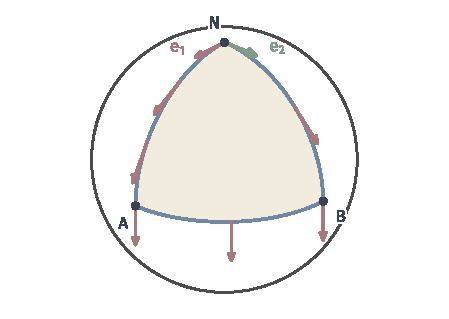
\includegraphics[width=76mm]{figures/04-spaces-measures-and-geometry/04-manifolds/matplotlib/riem-octant-transport/figure.pdf}
  \caption{球面八分之一三角形$N\to A\to B\to N$（黄色）上的平行移动。红箭头是例~\ref{ex:riem-sphere-transport}给出的向量$V(t)$，它沿每段大圆保持与路线的固定夹角；回到$N$时变为绿箭头$\bm e_2$，与初始的$\bm e_1$成直角。}
  \label{fig:riem-octant-transport}
\end{BookInlineFigure}

转角恰好等于这块球面三角形的面积$4\pi/8=\pi/2$。这个巧合在下面的例子中再次出现，第~\ref{sec:riem-curvature}节将用曲率解释。

\begin{example}[沿纬线的平行移动]
\label{ex:riem-latitude-transport}
沿过$p=(0,\tfrac35,\tfrac45)$的纬线搬运一个切向量。记$\theta_0$为$p$的极角，
\[
\sin\theta_0=\tfrac35,\qquad\cos\theta_0=\tfrac45 .
\]
路线取$(\theta,\phi)=(\theta_0,\tfrac\pi2+t)$，$t\in[0,2\pi]$。此时$\dot\theta=0$、$\dot\phi=1$，方程~\eqref{eq:riem-parallel-equation}化为
\[
\dot V_\theta=\sin\theta_0\cos\theta_0\,V_\phi,\qquad\dot V_\phi=-\cot\theta_0\,V_\theta .
\]

$\partial_\phi$的长度是$\sin\theta_0$，改用单位向量的分量会更清楚。令
\[
\bm e_\theta=\partial_\theta,\qquad\bm e_\phi=\frac{\partial_\phi}{\sin\theta_0},\qquad V=a\,\bm e_\theta+b\,\bm e_\phi ,
\]
则$V_\theta=a$，$V_\phi=b/\sin\theta_0$，代入得到
\[
\dot a=\cos\theta_0\,b,\qquad\dot b=-\cos\theta_0\,a .
\]

这是匀速旋转的方程。取初值$a(0)=1$、$b(0)=0$，也就是$p$处指向南方的单位向量，解为
\[
a(t)=\cos(\tfrac45t),\qquad b(t)=-\sin(\tfrac45t).
\]

绕一圈回到$p$时$t=2\pi$，$\tfrac45t=\tfrac{8\pi}5$，于是
\[
a(2\pi)=\cos\tfrac{2\pi}5\approx0.309,\qquad b(2\pi)=\sin\tfrac{2\pi}5\approx0.951 .
\]
向量从$\bm e_\theta$朝$\bm e_\phi$方向转过了$\tfrac{2\pi}5$。北极冠的面积是$2\pi(1-\cos\theta_0)=\tfrac{2\pi}5$，转角再次等于所围面积。
\end{example}

纬线的例子还可以用一张平面图来理解。沿纬线作球面的切锥，切点处锥面与球面有相同的切平面。对沿纬线的向量场，平行的条件只是“$\dot V$垂直于切平面”，所以在球面上平行与在切锥上平行是同一个条件。切锥可以摊平成平面扇形，半径$\tan\theta_0=\tfrac34$，圆心角$2\pi\cos\theta_0=\tfrac{8\pi}5$。在摊平的扇形上，平行向量就是常向量。

图~\ref{fig:riem-latitude-transport}(b)就是这个扇形：红箭头在平面上始终平行，$p$在扇形的两条边上各出现一次。扇形的缺口恰好是$\tfrac{2\pi}5$，这正是绕一圈的转角。

\begin{BookInlineFigure}
  \centering
  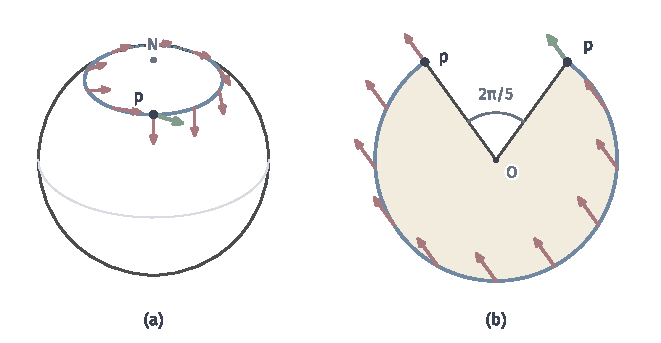
\includegraphics[width=112mm]{figures/04-spaces-measures-and-geometry/04-manifolds/matplotlib/riem-latitude-transport/figure.pdf}
  \caption{沿纬线的平行移动。(a)过$p=(0,\tfrac35,\tfrac45)$的纬线（蓝色）上，红箭头是从向南的单位向量出发平行移动的结果，绕一圈回到$p$时变为绿箭头，转过$\tfrac{2\pi}5$。(b)切锥摊平成的扇形，圆心角$\tfrac{8\pi}5$，缺口$\tfrac{2\pi}5$，纬线是外圆弧，$O$是锥顶。沿纬线的平行向量在扇形上是常向量，两条边是锥面上同一条母线。}
  \label{fig:riem-latitude-transport}
\end{BookInlineFigure}

\paragraph{与映射的微分比较}
第~\ref{chap:manifold-maps}章中，光滑映射$F:M\to N$在每点诱导线性映射$\mathrm dF_p:T_pM\to T_{F(p)}N$。平行移动$P_\gamma$也是切空间之间的线性映射，但二者的输入完全不同，表~\ref{tab:riem-transport-vs-differential}列出了对照。

\begin{BookInlineTable}
  \centering
  \begin{tabular}{lll}
    \toprule
    & 微分$\mathrm dF_p$ & 平行移动$P_\gamma$\\
    \midrule
    需要的输入 & 点映射$F$ & 曲线$\gamma$与联络\\
    是否需要度量 & 不需要 & 取Levi-Civita联络时需要\\
    依赖的范围 & $F$在$p$附近的取值 & 整条曲线\\
    \bottomrule
  \end{tabular}
  \caption{切空间之间的两种线性映射。}
  \label{tab:riem-transport-vs-differential}
\end{BookInlineTable}

在欧氏平面上取绕原点旋转角$\alpha$的映射$F$，则$\mathrm dF_p\bm v=\bm R_\alpha\bm v$，向量随之转过$\alpha$。而沿任何从$p$到$F(p)$的曲线作平行移动，得到的都是$\bm v$本身。两者都把$T_pM$映到$T_{F(p)}M$，结果却相差一个旋转。后面讨论等距映射与Lie群作用时，需要分清向量是“被映射带过去”还是“沿路径搬过去”的。

\section{测地线的初值问题}
\label{sec:riem-geodesic-ivp}

在平面上，“一直向前走”就是沿直线匀速运动，加速度为零。在球面上照搬这个说法会出问题：从$p=(1,0,0)$沿切方向$v=(0,1,0)$走直线$p+tv$，长度$\sqrt{1+t^2}$大于$1$，立刻离开球面。沿赤道$\gamma(t)=(\cos t,\sin t,0)$匀速前进则始终留在球面上，它的环境加速度$\ddot\gamma=-\gamma$不为零，却完全指向球面法向，只是“贴住球面”所必需的。沿球面没有转弯，意味着加速度的切向部分为零，也就是速度的协变导数为零。

\begin{definition}[测地线]
\label{def:riem-geodesic}
黎曼流形$(M,g)$上的光滑曲线$\gamma:I\to M$（$I$为区间）若满足
\[
\frac{D\dot\gamma}{\mathrm dt}=0,
\]
其中协变导数取Levi-Civita联络，就称$\gamma$为\term{测地线}（geodesic）。换言之，测地线的速度沿它自身平行移动。
\end{definition}

由定理~\ref{thm:riem-transport-isometry}，速度的长度沿测地线不变，所以测地线总是匀速的。这也意味着“测地线”是带参数化的概念：赤道换成非匀速参数化$t\mapsto(\cos t^3,\sin t^3,0)$，像集不变，速度大小却在变化，因此不再满足定义；只有仿射换元$t=as+b$保持测地线方程。本节先研究由初始位置和初始速度确定测地线的微分方程，再用指数映射把从一点出发的所有测地线汇总起来。

\subsection{测地线方程}
\label{sec:riem-geodesic-equation}

在坐标图中写$\gamma(t)$的坐标为$x(t)$，则$\dot\gamma=\sum_j\dot x^j\partial_j$。在式\eqref{eq:riem-covariant-derivative-along-curve}中取$V=\dot\gamma$，即$V^j=\dot x^j$，测地线条件化为
\begin{equation}
\ddot x^k(t)+\sum_{i,j=1}^n\Gamma^k_{i,j}\bigl(x(t)\bigr)\,\dot x^i(t)\,\dot x^j(t)=0,\qquad k=1,\ldots,n .
\label{eq:riem-geodesic-equation}
\end{equation}
与平行移动方程\eqref{eq:riem-parallel-equation}不同，这里系数依赖未知的$x(t)$，方程关于速度是二次的，因此是非线性方程。

\begin{example}[极坐标中的直线与球面上的大圆]
\label{ex:riem-geodesic-examples}
欧氏平面的极坐标中，由例~\ref{ex:riem-christoffel-examples}，测地线方程为
\[
\ddot r-r\dot\theta^2=0,\qquad\ddot\theta+\frac2r\dot r\dot\theta=0 .
\]
直线$x=1$匀速参数化为$y=t$，对应$r=\sqrt{1+t^2}$、$\theta=\arctan t$。计算得$\dot r=t(1+t^2)^{-1/2}$、$\ddot r=(1+t^2)^{-3/2}$、$\dot\theta=(1+t^2)^{-1}$、$\ddot\theta=-2t(1+t^2)^{-2}$，代入两式均为零。直线在直角坐标中的方程$\ddot x=\ddot y=0$，在极坐标中出现了Christoffel项。

单位球面上，方程为
\[
\ddot\theta-\sin\theta\cos\theta\,\dot\phi^2=0,\qquad\ddot\phi+2\cot\theta\,\dot\theta\dot\phi=0 .
\]
赤道$\theta=\pi/2$、$\phi=t$满足两式，是测地线。纬线$\theta=\theta_0\neq\pi/2$、$\phi=t$使第一式左端等于$-\sin\theta_0\cos\theta_0\neq0$，所以不是测地线：沿北半球的纬线匀速前进，需要一直向北侧转弯。
\end{example}

\paragraph{局部存在唯一与初值依赖}
把二阶方程改写成关于$(x,\dot x)$的一阶系统$\dot x=w$、$\dot w^k=-\sum_{i,j}\Gamma^k_{i,j}(x)w^iw^j$，右端是$(x,w)$的光滑函数。对这类方程，下面的结论成立，证明同样归入前面所引的卷六相应章节。

\begin{theorem}[光滑常微分方程的局部理论]
\label{thm:riem-smooth-ode}
设$W\subseteq\mathbb R^m$开，$F:W\to\mathbb R^m$光滑。则对每个$y_0\in W$：
\begin{enumerate}
\item 存在$\varepsilon>0$及唯一的解$y:(-\varepsilon,\varepsilon)\to W$，满足$\dot y=F(y)$、$y(0)=y_0$；
\item 两个解在公共定义区间上若有一个时刻取值相同，则在整个公共区间上相同，因而所有解可以拼成唯一的最大解，其定义区间是包含$0$的开区间；
\item 最大解$y(t;y_0)$关于$(t,y_0)$光滑，所有使其有定义的$(t,y_0)$构成开集；
\item 若最大解的定义区间右端点$t^+$有限，则当$t\to t^+$时$y(t)$终将离开$W$的每个紧子集。
\end{enumerate}
\end{theorem}

应用到测地线方程，得到：对每个$p\in M$和$v\in T_pM$，存在唯一的最大测地线$\gamma_v:I_v\to M$，满足$\gamma_v(0)=p$、$\dot\gamma_v(0)=v$，其中$I_v$是包含$0$的开区间。跨图时的拼接与平行移动相同，由唯一性保证一致。光滑依赖说明，初始速度稍有变化，测地线在有限时间内的位置也只稍有变化。

\paragraph{初始速度与时间的换算}
初始速度放大$c$倍，等价于把时间加快$c$倍：对$c\neq0$，$t\mapsto\gamma_v(ct)$满足测地线方程，初值为$p$与$cv$，所以
\begin{equation}
\gamma_{cv}(t)=\gamma_v(ct),\qquad t\in I_{cv}=\tfrac1cI_v .
\label{eq:riem-geodesic-rescaling}
\end{equation}
验证只需注意方程\eqref{eq:riem-geodesic-equation}的每一项关于时间导数是二次齐次的：$\ddot x$与$\dot x^i\dot x^j$都乘上$c^2$。

\paragraph{局部解未必能延拓到所有时间}
定理~\ref{thm:riem-smooth-ode}只保证解在某个时间区间内存在。在开单位球$M=\{x\in\mathbb R^n:\lVert x\rVert_2<1\}$上取欧氏度量，测地线是匀速直线。从原点以速度$2\bm e_1$出发，$\gamma(t)=2t\bm e_1$只在$t\in(-1/2,1/2)$内留在$M$中，最大定义区间是有限的；这正是结论(4)所说的“离开每个紧子集”。完整的单位球面上则不同，大圆对所有实数时间都有定义。测地线能否延拓到所有时间，取决于流形的整体性质，第~\ref{sec:riem-shortest-paths}节的Hopf--Rinow定理回答这个问题。

\subsection{黎曼指数映射}
\label{sec:riem-exponential-map}

从一点$p$出发，每个初始速度$v$给出一条测地线。把“沿$v$方向走单位时间到达哪里”记录下来，就得到从切空间$T_pM$到流形的一个映射。它把$p$附近的点用一个切向量来标记，类似于在地图上用“方向和距离”标记位置。

\begin{definition}[黎曼指数映射]
\label{def:riem-exponential-map}
对$p\in M$，令$\mathcal E_p=\{v\in T_pM:1\in I_v\}$为测地线$\gamma_v$至少存在到时刻$1$的初速度全体。定义
\[
\exp_p:\mathcal E_p\to M,\qquad\exp_p(v)=\gamma_v(1),
\]
称为$p$处的\term{黎曼指数映射}（Riemannian exponential map）。
\end{definition}

由式\eqref{eq:riem-geodesic-rescaling}，若$v\in\mathcal E_p$且$0\leq t\leq1$，则$tv\in\mathcal E_p$，并且
\[
\exp_p(tv)=\gamma_{tv}(1)=\gamma_v(t).
\]
所以沿射线$t\mapsto tv$的像正是测地线$\gamma_v$，定义域$\mathcal E_p$关于原点呈星形。由定理~\ref{thm:riem-smooth-ode}的结论(3)，$\mathcal E_p$是包含$0$的开集，$\exp_p$在其上光滑。

\begin{theorem}[指数映射的局部可逆性]
\label{thm:riem-exp-local-diffeo}
对每个$p\in M$，$d(\exp_p)_0:T_0(T_pM)\cong T_pM\to T_pM$是恒等映射。因此存在$0$在$T_pM$中的开邻域$V$和$p$在$M$中的开邻域$U$，使$\exp_p:V\to U$是微分同胚。
\end{theorem}

\begin{proof}
线性空间$T_pM$在$0$处的切空间可以认同为$T_pM$本身。对$v\in T_pM$，曲线$t\mapsto tv$在$t=0$的速度是$v$，它在$\exp_p$下的像是$\gamma_v(t)$，速度为$\dot\gamma_v(0)=v$。由链式法则，$d(\exp_p)_0(v)=v$。微分在一点可逆，由反函数定理即得局部微分同胚；反函数定理的欧氏形式可参考\BookChapterRef{chap:implicit-inverse-functions}{卷二“隐函数与反函数”章}，它在流形上的形式见第~\ref{chap:manifold-relations}章。
\end{proof}

若$V$还可以取为关于原点星形的，例如以$0$为心的球$\{v:\lVert v\rVert_g<\varepsilon\}$，则称像集$U=\exp_p(V)$为$p$的\term{正常邻域}（normal neighborhood）。在正常邻域中，每个点$q$都唯一地写成$q=\exp_p(v)$，$v\in V$，从$p$到$q$有一条“径向”测地线$t\mapsto\exp_p(tv)$。取$T_pM$的一组标准正交基把$v$写成坐标，就得到$U$上的一组坐标，称为$p$处的法坐标。

\begin{example}[单位球面的指数映射]
\label{ex:riem-sphere-exp}
单位球面$\mathbb S^{n}\subseteq\mathbb R^{n+1}$上，取$p$与$v\perp p$，$r=\lVert v\rVert_2>0$。曲线$\gamma(t)=\cos(tr)\,p+\sin(tr)\,v/r$满足$\lVert\gamma(t)\rVert_2=1$，$\gamma(0)=p$，$\dot\gamma(0)=v$，且$\ddot\gamma=-r^2\gamma$为纯法向，所以它是测地线。于是$\mathcal E_p=T_p\mathbb S^n$，并且
\[
\exp_p(v)=\cos\lVert v\rVert_2\,p+\frac{\sin\lVert v\rVert_2}{\lVert v\rVert_2}\,v,\qquad\exp_p(0)=p .
\]
所有长度为$\pi$的初速度都到达对跖点$-p$，所以$\exp_p$不是单射；在开球$\lVert v\rVert_2<\pi$上它是到$\mathbb S^n\setminus\{-p\}$的微分同胚。可见即使指数映射处处有定义，可逆性也只是局部的。
\end{example}

\paragraph{与矩阵指数的区别}
第~\ref{chap:lie-groups}章会在矩阵Lie群上用矩阵指数$e^{\bm A}=\sum_k\bm A^k/k!$把单位元处的切向量变成群元素。两者都叫“指数”，都从切空间出发、在零点处微分为恒等，但来源不同：黎曼指数映射由度量经Levi-Civita联络确定，换一个度量就会改变；矩阵指数只由群的乘法确定，不需要度量。在带特殊度量的某些群上二者可以一致，这需要单独验证，不能仅凭名称相同就互相替代。

\section{给定端点的最短路径}
\label{sec:riem-shortest-paths}

上一节固定的是起点和初始速度，本节固定的是两个端点。问题变成：在所有连接$p$与$q$的分段光滑曲线中，长度能否达到内在距离$d_g(p,q)$，达到时曲线是什么样子。我们分三步回答。先比较长度与能量，说明长度最短且匀速的曲线满足测地线方程；再证明足够短的测地线确实最短；最后陈述保证最短曲线存在的整体条件。每一步的结论都比前一步的要求多，不能互相替代。

\subsection{长度与能量的变分}
\label{sec:riem-length-energy-variation}

长度的被积函数$\lVert\dot\gamma\rVert_g$含有平方根，直接求导不便，而且长度对任何单调换参数都不变，同一条路线有无穷多种参数化都是“最优”的。常用的办法是改用能量。对$\gamma:[a,b]\to M$，定义\term{曲线能量}（energy of a curve）
\begin{equation}
E(\gamma)=\frac12\int_a^b\lVert\dot\gamma(t)\rVert_g^2\,\mathrm dt .
\label{eq:riem-energy}
\end{equation}

\paragraph{长度与能量的比较}
由Cauchy--Schwarz不等式，把$\lVert\dot\gamma\rVert_g$看成与常函数$1$作内积：
\[
L_g(\gamma)^2=\Bigl(\int_a^b1\cdot\lVert\dot\gamma\rVert_g\,\mathrm dt\Bigr)^2\leq(b-a)\int_a^b\lVert\dot\gamma\rVert_g^2\,\mathrm dt .
\]
右端等于$2(b-a)E(\gamma)$，所以
\begin{equation}
L_g(\gamma)^2\leq2(b-a)E(\gamma),
\label{eq:riem-length-energy}
\end{equation}
等号成立当且仅当$\lVert\dot\gamma\rVert_g$在$[a,b]$上几乎处处为常数，即曲线匀速。

因此在固定时间区间上，走同一条路线时忽快忽慢只会增加能量。例如在实数轴上走$[0,1]$这段路线，$x(t)=t^2$，$t\in[0,1]$，长度$L=1$，能量却是
\[
E=\frac12\int_0^1(2t)^2\,\mathrm dt=\frac23 .
\]
匀速的$x(t)=t$给出$E=\tfrac12=L^2/2$，式~\eqref{eq:riem-length-energy}取等号。能量最小的曲线必然匀速。速度处处非零的曲线可以重新参数化为匀速，所以在匀速曲线之间比较能量，等同于比较长度。

\paragraph{能量的驻定条件}
现在考察端点固定的扰动。设$\gamma$落在一张坐标图内，坐标为$x(t)$；取光滑的$h:[a,b]\to\mathbb R^n$，$h(a)=h(b)=0$，对足够小的$\varepsilon$令$x_\varepsilon=x+\varepsilon h$。若对所有这样的$h$都有
\[
\frac{\mathrm d}{\mathrm d\varepsilon}E(\gamma_\varepsilon)\Big|_{\varepsilon=0}=0,
\]
就称$\gamma$是能量的驻定曲线。

能量的被积函数是
\[
\mathscr L(x,\dot x)=\frac12\sum_{i,j}g_{i,j}(x)\,\dot x_i\dot x_j .
\]
对这类积分，所用的结论是Euler--Lagrange关系：若$\mathscr L$光滑，$x$为$C^2$曲线，则$x$在端点固定的扰动下驻定当且仅当
\begin{equation}
\frac{\partial\mathscr L}{\partial x_k}-\frac{\mathrm d}{\mathrm dt}\frac{\partial\mathscr L}{\partial\dot x_k}=0,\qquad k=1,\ldots,n .
\label{eq:riem-euler-lagrange}
\end{equation}
它的推导是对$\varepsilon$求导后分部积分，边界项因$h(a)=h(b)=0$消失，再由$h$的任意性得到被积系数为零；一般泛函的变分理论可参考\BookChapterRef{chap:functional-optimization-variation}{卷五“泛函优化与变分”章}。

把能量代入。对$x_k$和$\dot x_k$分别求偏导，
\[
\frac{\partial\mathscr L}{\partial x_k}=\frac12\sum_{i,j}\partial_kg_{i,j}\,\dot x_i\dot x_j,\qquad
\frac{\partial\mathscr L}{\partial\dot x_k}=\sum_jg_{k,j}\dot x_j .
\]

后一式对时间求导，用链式法则：
\[
\frac{\mathrm d}{\mathrm dt}\sum_jg_{k,j}\dot x_j=\sum_jg_{k,j}\ddot x_j+\sum_{i,j}\partial_ig_{k,j}\,\dot x_i\dot x_j .
\]
第二项对$i,j$对称化，写成$\frac12\sum_{i,j}(\partial_ig_{k,j}+\partial_jg_{k,i})\dot x_i\dot x_j$。

代回式~\eqref{eq:riem-euler-lagrange}并取负号，得到
\[
\sum_jg_{k,j}\ddot x_j+\frac12\sum_{i,j}\bigl(\partial_ig_{k,j}+\partial_jg_{k,i}-\partial_kg_{i,j}\bigr)\dot x_i\dot x_j=0 .
\]
括号恰是式~\eqref{eq:riem-christoffel}中的组合。两边乘$\bm G^{-1}$，得到测地线方程~\eqref{eq:riem-geodesic-equation}。曲线跨越多张图时，用支撑在单张图内的扰动逐段推导，结论相同。

单位球面可以这样快速验算。被积函数是
\[
\mathscr L=\tfrac12\bigl(\dot\theta^2+\sin^2\theta\,\dot\phi^2\bigr).
\]

对$\theta$和对$\phi$的方程分别是
\[
\ddot\theta-\sin\theta\cos\theta\,\dot\phi^2=0,\qquad
\frac{\mathrm d}{\mathrm dt}\bigl(\sin^2\theta\,\dot\phi\bigr)=0 .
\]
第二式展开后就是例~\ref{ex:riem-geodesic-examples}中的第二个方程。

这样得到两条结论。光滑曲线是能量的驻定曲线，当且仅当它是测地线。若匀速曲线在所有连接相同端点的曲线中长度最短，则它也是能量最小的，因而是测地线。长度本身的驻定曲线则只确定路线、不确定参数化：长度的Euler--Lagrange方程对任意换参数都成立，换成匀速参数后才是测地线方程。

\paragraph{驻定不等于最短}
驻定条件只是一阶条件，类似卷一中导数为零的点不一定是最小值点。完整单位圆上，从$(1,0)$到$(0,-1)$，顺时针的短弧长$\pi/2$，逆时针的长弧长$3\pi/2$，二者匀速参数化后都是测地线，只有前者最短。单位球面上沿大圆从$p$出发走过对跖点再继续，同样是测地线，却比反方向的另一段大圆弧长。驻定曲线是否最短，还要额外比较。

\subsection{局部最短性}
\label{sec:riem-local-minimality}

上面的反例都发生在曲线较长时。下面证明：足够短的测地线一定最短。论证用到正常邻域中径向与“横向”方向的正交关系。平面上，同心圆与半径处处垂直；下面的Gauss引理说明，在指数映射的图像里同样如此。

\begin{lemma}[Gauss引理]
\label{lem:riem-gauss-lemma}
设$\exp_p$在$T_pM$中以$\bm 0$为心、半径$\varepsilon$的球$B_\varepsilon(\bm 0)$上是微分同胚。对$\bm v\in B_\varepsilon(\bm 0)$，$\bm v\neq\bm 0$，以及任意$\bm w\in T_pM$，有
\begin{equation}
g\bigl(\mathrm d(\exp_p)_{\bm v}(\bm v),\,\mathrm d(\exp_p)_{\bm v}(\bm w)\bigr)=g_p(\bm v,\bm w).
\label{eq:riem-gauss-lemma}
\end{equation}
特别地，径向测地线的速度与由长度等于$\lVert\bm v\rVert_g$的切向量在$\exp_p$下的像组成的球面在交点处正交。
\end{lemma}

\begin{proof}
构造一族从$p$出发的测地线：对$t\in[0,1]$和足够小的$s$，令
\[
f(t,s)=\exp_p\bigl(t(\bm v+s\bm w)\bigr).
\]
$f$是光滑的，固定$s$时它是初速度为$\bm v+s\bm w$的测地线。记$T=\partial_tf$，$S=\partial_sf$，这是沿这族曲线的两个向量场。

我们需要两个事实。第一，$T$沿$t$方向的协变导数为零，这是测地线方程：$D_tT=0$。第二，$D_tS=D_sT$，这是无挠条件的结果。在坐标中，$D_tS$的$k$分量是
\[
\frac{\partial^2x_k}{\partial t\,\partial s}+\sum_{i,j}\Gamma^k_{i,j}\frac{\partial x_i}{\partial t}\frac{\partial x_j}{\partial s},
\]
由$\Gamma^k_{i,j}$的对称性，它关于$t,s$对称。

对$g(T,S)$关于$t$求导，用度量相容和上面两个事实：
\[
\partial_t\,g(T,S)=g(D_tT,S)+g(T,D_tS)=g(T,D_sT).
\]

右端等于$\tfrac12\partial_s\,g(T,T)$。测地线匀速，所以$g(T,T)$等于初速度的长度平方$\lVert\bm v+s\bm w\rVert_g^2$，与$t$无关。取$s=0$，得到
\[
\partial_t\,g(T,S)\big|_{s=0}=\tfrac12\frac{\mathrm d}{\mathrm ds}\lVert\bm v+s\bm w\rVert_g^2\Big|_{s=0}=g_p(\bm v,\bm w).
\]

右端是常数。在$t=0$处，$f(0,s)=p$与$s$无关，所以$S(0,0)=\bm 0$，$g(T,S)$从$0$开始。沿$t$积分到$t=1$，得到
\[
g(T,S)\big|_{(1,0)}=g_p(\bm v,\bm w).
\]
而$T(1,0)=\mathrm d(\exp_p)_{\bm v}(\bm v)$，$S(1,0)=\mathrm d(\exp_p)_{\bm v}(\bm w)$，这就是式~\eqref{eq:riem-gauss-lemma}。

取$\bm w$与$\bm v$垂直，右端为零，所以径向方向与测地球面垂直。
\end{proof}

称$\exp_p(B_\varepsilon(\bm 0))$为$p$的半径$\varepsilon$的测地球。Gauss引理把图~\ref{fig:riem-exp-map}(c)的分解变成了等式：速度分解成径向和横向两部分，二者互相垂直，勾股定理可以用。

\begin{theorem}[径向测地线的最短性]
\label{thm:riem-radial-minimizing}
设$\exp_p$在$B_\varepsilon(\bm 0)\subseteq T_pM$上是微分同胚，$q=\exp_p(\bm v)$，$\lVert\bm v\rVert_g<\varepsilon$。则径向测地线$\sigma(t)=\exp_p(t\bm v)$，$t\in[0,1]$，长度为$\lVert\bm v\rVert_g$，并且任何从$p$到$q$的分段光滑曲线长度都不小于$\lVert\bm v\rVert_g$。因此
\begin{equation}
d_g(p,q)=\lVert\bm v\rVert_g .
\label{eq:riem-radial-distance}
\end{equation}
\end{theorem}

\begin{proof}
$\sigma$是初速度为$\bm v$的测地线，匀速，所以$L_g(\sigma)=\lVert\bm v\rVert_g$。设$\gamma:[a,b]\to M$是任一从$p$到$q$的分段光滑曲线。可以假设$\gamma$在$t>a$时不再经过$p$，否则从最后一次经过$p$的时刻开始考虑，长度只会变小。

先设$\gamma$始终留在测地球中。对$t>a$写
\[
\gamma(t)=\exp_p\bigl(\rho(t)\bm u(t)\bigr),\qquad\rho(t)>0,\quad\lVert\bm u(t)\rVert_g=1 .
\]

由链式法则，
\[
\dot\gamma=\mathrm d(\exp_p)\bigl(\dot\rho\,\bm u+\rho\,\dot{\bm u}\bigr),
\]
其中$\dot{\bm u}\perp\bm u$，因为$\lVert\bm u\rVert_g$恒为$1$。在式~\eqref{eq:riem-gauss-lemma}中取$\bm v=\rho\bm u$、$\bm w=\bm u$，得到$\mathrm d(\exp_p)(\bm u)$的长度为$1$。再取$\bm w=\rho\dot{\bm u}$，得到它与$\mathrm d(\exp_p)(\rho\dot{\bm u})$正交。

于是两部分互相垂直，由勾股定理，
\[
\lVert\dot\gamma\rVert_g^2=\dot\rho^2+\bigl\lVert\mathrm d(\exp_p)(\rho\dot{\bm u})\bigr\rVert_g^2\geq\dot\rho^2 .
\]

积分，并让积分下限趋于$a$（此时$\rho\to0$），得到
\[
L_g(\gamma)\geq\int_a^b\lvert\dot\rho\rvert\,\mathrm dt\geq\rho(b)-\lim_{t\to a^+}\rho(t)=\lVert\bm v\rVert_g .
\]

若$\gamma$离开测地球，它在离开前必须先到达每个半径$\delta<\varepsilon$的测地球面。对满足$\lVert\bm v\rVert_g<\delta<\varepsilon$的$\delta$，把上面的论证用于从$p$到第一次到达半径$\delta$球面的那一段，得到$L_g(\gamma)\geq\delta>\lVert\bm v\rVert_g$。两种情形合起来即得结论。
\end{proof}

证明中的不等式还给出等号条件：长度恰为$\lVert\bm v\rVert_g$的曲线必须$\rho$单调、横向分量为零，也就是沿径向走。所以测地球内$p$到$q$的最短曲线，除参数化外只有径向测地线这一条。

定理比较的是从中心$p$出发的所有曲线，包括离开测地球的曲线，所以结论是真正的距离等式。它对测地球中任意两点之间的连线并不直接给出结论：两点都不是中心时，需要更小的凸正常邻域，在那里任意两点由唯一一条留在邻域内的最短测地线连接。这一进一步的局部结论的证明较长，读者可查阅Lee的教材\scite{math-lee2018riemannian}。称长度等于两端点内在距离的测地线为\term{最短测地线}（minimizing geodesic）。

\paragraph{局部最短不意味着全局最短或唯一}
定理~\ref{thm:riem-radial-minimizing}给出：每条测地线的足够短的一段都是最短测地线。但整条测地线可以不是最短的。取半径为$1$的圆柱面$\{(x,y,z):x^2+y^2=1\}$，曲线$t\mapsto(\cos t,\sin t,ct)$匀速，环境加速度$(-\cos t,-\sin t,0)$沿法向，所以这些螺旋线是测地线。

考虑连接$p_0=(1,0,0)$与$p_1=(1,0,\pi)$的曲线。竖直线段长$\pi$。绕$k$圈的螺旋线$t\mapsto(\cos t,\sin t,\tfrac{t}{2k})$，$t\in[0,2\pi k]$，速率是$\sqrt{1+1/(4k^2)}$，长度为
\[
L_k=2\pi k\sqrt{1+\frac1{4k^2}}=\pi\sqrt{4k^2+1}.
\]
$k=1,2$时分别是$\pi\sqrt5\approx7.02$和$\pi\sqrt{17}\approx12.95$，反向绕圈的情形相同。连接同一对端点的测地线有无穷多条，局部都是最短的，只有竖直线段全局最短。

图~\ref{fig:riem-cylinder-geodesics}把这些曲线放到圆柱展开的平面上：$p_1$有无穷多个“复本”，每条测地线就是通向其中一个复本的直线段。球面的对跖点则说明，最短测地线本身也可以不唯一：所有从$p$到$-p$的半个大圆都是最短的。

\begin{BookInlineFigure}
  \centering
  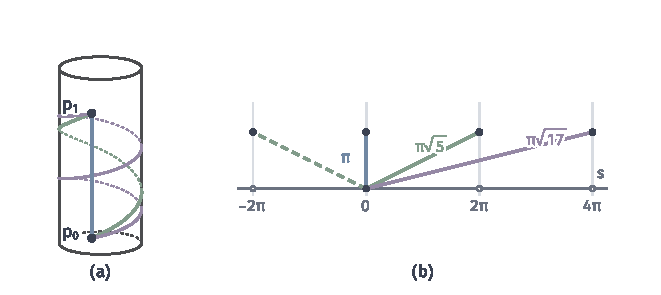
\includegraphics[width=112mm]{figures/04-spaces-measures-and-geometry/04-manifolds/matplotlib/riem-cylinder-geodesics/figure.pdf}
  \caption{圆柱面上连接同一对点的多条测地线。(a)单位圆柱上的$p_0=(1,0,0)$、$p_1=(1,0,\pi)$，蓝色竖直线段长$\pi$，绿色、紫色分别绕$1$圈、$2$圈。(b)沿圆周方向展开，竖线是$s=2\pi k$处$p_0$与$p_1$的复本，每条测地线是从原点到一个复本的线段，长度分别为$\pi$、$\pi\sqrt5$、$\pi\sqrt{17}$；虚线是反向绕圈的情形。}
  \label{fig:riem-cylinder-geodesics}
\end{BookInlineFigure}

\subsection{最短路径的存在}
\label{sec:riem-shortest-existence}

局部最短性只回答“短距离内测地线就是最短路”，不回答相距较远的两点之间是否有最短路。图~\ref{fig:riem-punctured-plane}的穿孔平面表明，答案可以是否定的：缺口使逼近下确界的曲线序列没有极限。排除这类缺口的条件是度量完备性。

\begin{theorem}[Hopf--Rinow定理]
\label{thm:riem-hopf-rinow}
设$(M,g)$是有限维、连通、无边界的黎曼流形。下列条件等价：
\begin{enumerate}
\item 度量空间$(M,d_g)$完备；
\item $M$是\term{测地完备}（geodesically complete）的，即每条测地线都能延拓到全体实数时间；
\item 存在某一点$p$，使$\exp_p$在整个$T_pM$上有定义；
\item $M$中有界闭集都是紧集。
\end{enumerate}
满足这些条件时，任意两点$p,q\in M$之间存在长度为$d_g(p,q)$的最短测地线。
\end{theorem}

这一定理称为\term{Hopf--Rinow定理}（Hopf--Rinow theorem）。证明需要依次比较几种完备性，篇幅较长，读者可查阅前引教材。它的机制可以这样理解：条件(3)使从$p$出发的每个方向都能一直走下去。对远处的点$q$，在$p$附近的测地球面上取与$q$距离最小的点，沿指向它的方向走测地线，可以证明这条测地线一直“对准”$q$，走过距离$d_g(p,q)$时恰好到达$q$。完备性保证这一过程不会中途掉进缺口。

\paragraph{条件的作用}
紧的无边界黎曼流形总是完备的：紧度量空间中的Cauchy列有收敛子列，从而本身收敛（第~\ref{chap:metric-spaces}章）。所以球面、环面等闭曲面上任意两点之间都有最短测地线。穿孔平面与开单位球不完备：前者中趋于原点的点列是Cauchy列却不收敛，后者中直线测地线在有限时间到达缺失的边界。

定理的最后结论只是充分条件。开单位球不完备，但它是凸集，任意两点之间的线段留在球内，是最短测地线；穿孔平面则连这一点也做不到。所以“任意两点都有最短路”不能反推完备性，而缺少完备性时，最短路是否存在要具体判断。

\paragraph{存在与唯一}
Hopf--Rinow定理保证存在，不保证唯一。球面对跖点之间有无穷多条最短测地线，圆柱面上位于同一水平圆的对径点之间有两条。存在性也不能由测地线方程的局部存在唯一性推出：后者固定的是初始速度，回答的是“从这个方向出发会走到哪里”；端点问题要找的是“哪个初始速度能恰好到达$q$且最短”，这需要比较全部路线，依赖流形的整体结构。

\section{曲率}
\label{sec:riem-curvature}

例~\ref{ex:riem-sphere-transport}中，球面上绕一圈平行移动回到起点，向量转过了$\pi/2$；平面上无论怎样绕，向量都不变。这个差别不是坐标造成的，而是两种几何本身不同。本节要找一个逐点定义、与坐标无关的量来检测它。思路是把绕圈缩小到无穷小：沿两个方向先后求协变导数，比较两种次序的结果。得到的曲率张量描述内在几何；最后再把它与曲面在环境空间中“看上去弯曲”的程度区分开。

\subsection{曲率张量与截面曲率}
\label{sec:riem-curvature-tensor}

在欧氏空间中，二阶偏导数可以交换次序。对向量场的协变导数，交换次序的差$\nabla_X\nabla_YZ-\nabla_Y\nabla_XZ$一般不为零，但其中有一部分来自方向场本身：即使在平面上，若$X,Y$不可交换，先沿$X$再沿$Y$与先沿$Y$再沿$X$也不会回到同一点。这部分差别由Lie括号$[X,Y]$描述，应当扣除。

\begin{definition}[黎曼曲率张量]
\label{def:riem-curvature-tensor}
设$\nabla$是$(M,g)$的Levi-Civita联络。对$X,Y,Z\in\mathfrak X(M)$定义
\begin{equation}
R(X,Y)Z=\nabla_X\nabla_YZ-\nabla_Y\nabla_XZ-\nabla_{[X,Y]}Z .
\label{eq:riem-curvature}
\end{equation}
$R$称为$(M,g)$的\term{黎曼曲率张量}（Riemann curvature tensor）。
\end{definition}

文献中曲率的符号约定不统一，有的教材把上式整体取负号。本书采用上式，在这一约定下单位球面的截面曲率为正，后面会核对。

\paragraph{曲率是逐点定义的}
式\eqref{eq:riem-curvature}的三项都含有导数，似乎需要知道$X,Y,Z$在一点附近的取值。实际上$R$对三个变量都按函数线性，所以$(R(X,Y)Z)(p)$只依赖$X_p,Y_p,Z_p$。以$Z$为例，把$fZ$代入，由乘积法则
\[
\nabla_X\nabla_Y(fZ)=(XYf)Z+(Yf)\nabla_XZ+(Xf)\nabla_YZ+f\nabla_X\nabla_YZ .
\]
交换$X,Y$后相减，中间两项抵消，第一项变为$([X,Y]f)Z$；而$\nabla_{[X,Y]}(fZ)=([X,Y]f)Z+f\nabla_{[X,Y]}Z$，恰好消去这一项，剩下$fR(X,Y)Z$。对$X$的函数线性可以类似验证，第三项$\nabla_{[X,Y]}Z$在其中同样负责抵消导数项；对$Y$的情形由$R(X,Y)=-R(Y,X)$得到。因此对点$p$处的切向量$u,v,w$可以写$R(u,v)w\in T_pM$。

\paragraph{坐标表示}
取坐标基场代入，Lie括号项消失，由$\nabla_{\partial_i}\nabla_{\partial_j}\partial_k=\nabla_{\partial_i}\bigl(\sum_m\Gamma^m_{j,k}\partial_m\bigr)$展开，得到$R(\partial_i,\partial_j)\partial_k=\sum_\ell R^\ell_{i,j,k}\partial_\ell$，其中
\begin{equation}
R^\ell_{i,j,k}=\partial_i\Gamma^\ell_{j,k}-\partial_j\Gamma^\ell_{i,k}+\sum_m\bigl(\Gamma^m_{j,k}\Gamma^\ell_{i,m}-\Gamma^m_{i,k}\Gamma^\ell_{j,m}\bigr).
\label{eq:riem-curvature-coordinates}
\end{equation}
曲率由度量的二阶导数决定。若在某组坐标中$\bm G$为常矩阵，则所有Christoffel符号为零，$R=0$。反过来，系数不为零并不说明曲率非零：极坐标中Christoffel符号不为零，平面的曲率仍为零，因为$R$是张量，在直角坐标中为零就在任何坐标中为零。

\paragraph{截面曲率}
$R$有三个输入，信息较多。最常用的标量是在一个二维切平面上读出的曲率。

\begin{definition}[截面曲率]
\label{def:riem-sectional-curvature}
设$u,v\in T_pM$线性无关，它们张成的平面$\Pi$的\term{截面曲率}（sectional curvature）为
\begin{equation}
K(\Pi)=K(u,v)=\frac{g\bigl(R(u,v)v,u\bigr)}{g(u,u)g(v,v)-g(u,v)^2}.
\label{eq:riem-sectional-curvature}
\end{equation}
\end{definition}

分母是$u,v$张成的平行四边形面积的平方，由Cauchy--Schwarz不等式，它在$u,v$线性无关时为正。可以证明分子在把$(u,v)$换成同一平面的另一组基时，与分母乘上相同的因子，所以$K$只依赖平面$\Pi$；这一点用到$g(R(u,v)w,z)$关于$(u,v)$和关于$(w,z)$都反对称的性质，这里不展开。二维流形每点只有一个切平面，截面曲率就是一个函数，称为\term{Gauss曲率}（Gaussian curvature）。一维流形没有二维切平面，式\eqref{eq:riem-curvature}中的$R$恒为零。

\begin{example}[单位球面的曲率]
\label{ex:riem-sphere-curvature}
用例~\ref{ex:riem-christoffel-examples}的系数$\Gamma^\theta_{\phi,\phi}=-\sin\theta\cos\theta$、$\Gamma^\phi_{\theta,\phi}=\Gamma^\phi_{\phi,\theta}=\cot\theta$计算$R(\partial_\theta,\partial_\phi)\partial_\phi$。由式\eqref{eq:riem-curvature-coordinates}，其$\theta$分量为
\begin{equation*}
\begin{aligned}
R^\theta_{\theta,\phi,\phi}&=\partial_\theta\Gamma^\theta_{\phi,\phi}-\partial_\phi\Gamma^\theta_{\theta,\phi}+\sum_m\bigl(\Gamma^m_{\phi,\phi}\Gamma^\theta_{\theta,m}-\Gamma^m_{\theta,\phi}\Gamma^\theta_{\phi,m}\bigr)\\
&=(\sin^2\theta-\cos^2\theta)-0+0-\cot\theta\cdot(-\sin\theta\cos\theta)=\sin^2\theta,
\end{aligned}
\end{equation*}
其中只有$m=\phi$的一项$\Gamma^\phi_{\theta,\phi}\Gamma^\theta_{\phi,\phi}$非零；同样可算出$\phi$分量为零。于是$R(\partial_\theta,\partial_\phi)\partial_\phi=\sin^2\theta\,\partial_\theta$，分子$g(R(\partial_\theta,\partial_\phi)\partial_\phi,\partial_\theta)=\sin^2\theta$，分母$1\cdot\sin^2\theta-0=\sin^2\theta$，所以$K=1$。半径为$a$的球面按同样计算得$K=1/a^2$：球越大，曲率越小，越接近平面。
\end{example}

\paragraph{小回路上的平行移动}
曲率与绕圈搬运的联系可以这样表述。在$p$处取线性无关的$u,v$，在法坐标中沿边长为$s$的小“平行四边形”回路（依次沿$su$、$sv$、$-su$、$-sv$方向）平行移动，记所得的线性映射为$P_s:T_pM\to T_pM$。则当$s\to0$时
\[
P_s(w)=w-s^2R(u,v)w+o(s^2),
\]
首项的符号随绕行方向和曲率符号约定而变。这里只说明机制，不给出证明：每条边上的平行移动可以展开到二阶，四段复合时一阶项相互抵消，二阶项中剩下的正是两种求导次序之差。在单位球面北极取$u=\bm e_1$、$v=\bm e_2$，由球面上$R(u,v)w=g(v,w)u-g(u,w)v$（可由例~\ref{ex:riem-sphere-curvature}的结果连同对称性推出）得$R(u,v)$把$v$映到$u$、把$u$映到$-v$，是切平面内转过直角的线性映射。所以小回路的效应是一个与所围面积$s^2$成比例的小转动。

\paragraph{局部曲率与整体回路}
曲率是局部量，有限回路的总效应还受整体形状影响，不能简单地把一点的曲率乘上面积。一个清楚的例子是锥面。从平面上剪去圆心角为$\alpha$（$0<\alpha<2\pi$）的扇形，把两条剪边粘合，再去掉顶点，得到的曲面每一小块都可以摊平成平面的一块，所以曲率处处为零。然而沿绕顶点一周的回路平行移动，在摊开的扇形中向量保持不变，经过粘合边时却要按扇形张角旋转一次，回到出发点时向量转过角$\alpha$。没有曲率的区域上，绕不可收缩的回路仍可以有非平凡的平行移动；这是拓扑与局部几何共同造成的。

\subsection{内在曲率与嵌入弯曲}
\label{sec:riem-intrinsic-extrinsic}

日常说一个曲面“弯”，通常指它在三维空间中的形状。黎曼曲率衡量的则是曲面内部的长度规则能否摊平成平面。这两件事不同：一张纸可以卷成圆柱而不拉伸、不起皱，纸上的长度与角度保持不变；却无法不拉伸地包住一个球。

\paragraph{平面与圆柱}
取半径为$a$的圆柱面，局部参数化为
\begin{equation*}
\Phi(s,z)=(a\cos(s/a),a\sin(s/a),z),\qquad s\in(0,2\pi a).
\end{equation*}两列切向量为$(-\sin(s/a),\cos(s/a),0)$与$(0,0,1)$，都是单位向量且互相正交，所以诱导度量$\bm G=\bm I$。在这组坐标中Christoffel符号全为零，曲率张量为零，截面曲率$K=0$。就内在几何而言，圆柱面的这一块与平面的一个矩形没有区别。

圆柱在环境中的弯曲由法向量的变化体现。单位法向量为$n(s,z)=(\cos(s/a),\sin(s/a),0)$，沿$s$方向的导数是$\frac1a(-\sin(s/a),\cos(s/a),0)$，大小$1/a$；沿$z$方向不变。这两个数$1/a$与$0$称为曲面在该点的\term{主曲率}（principal curvature），它们描述法向量沿各方向转动的快慢，属于嵌入的性质。对半径为$a$的球面，法向量$n=x/a$沿任何单位切方向的导数大小都是$1/a$，两个主曲率都是$1/a$。

两种曲面的Gauss曲率与主曲率之间有一个关系：对$\mathbb R^3$中的曲面，Gauss曲率等于两个主曲率之积。圆柱给出$\frac1a\cdot0=0$，球面给出$\frac1{a^2}$，与前面的内在计算一致。这一关系称为Gauss绝妙定理，这里不给出证明；它的意义是，主曲率依赖嵌入，它们的乘积却只由诱导度量决定。

\paragraph{为什么要区分}
一维的例子更极端。半径为$a$的圆在平面中明显弯曲，法向偏离切线的程度由曲率$1/a$描述；可它的黎曼曲率恒为零，任何一段弧都与一段直线等距。所以，“法向量在变”“切平面在转”都不能作为内在曲率非零的证据，坐标中度量系数随位置变化也不能。反过来，内在平坦也不意味着嵌入不弯，圆柱就是例子。

这一区分在由采样点估计几何时很重要。第~\ref{chap:manifold-recovery}章用切平面拟合局部点云时，点到切平面的偏离量由法向量的变化，即嵌入弯曲控制，在圆或圆柱上也会出现；它反映的是嵌入的主曲率，而不是内在截面曲率。估计误差的分析须保持这一区分。

\section{等距映射}
\label{sec:riem-isometries}

前面各节都在一个黎曼流形内部讨论。圆柱的例子已经提出了比较两个黎曼流形的问题：圆柱的一块与平面的一块“内在几何相同”，这句话要怎样准确表述？第~\ref{chap:manifold-relations}章用微分同胚表达两个流形具有相同的光滑结构，但微分同胚可以任意拉伸长度。这里要求映射在每个切空间上保持内积。

\paragraph{保持内积的条件}
设$(M,g)$与$(N,h)$是黎曼流形，$F:M\to N$光滑。映射的微分$dF_p:T_pM\to T_{F(p)}N$把切向量从$p$带到$F(p)$。我们要求：任取$p\in M$及$u,v\in T_pM$，
\begin{equation}
g_p(u,v)=h_{F(p)}\bigl(dF_pu,\,dF_pv\bigr).
\label{eq:riem-isometry-condition}
\end{equation}
右端是用$N$的度量量出的、被带过去的两个向量的内积，左端是原来的内积。在坐标中，若$F$的Jacobian矩阵为$\bm J$，条件就是$\bm G_M=\bm J^{\top}\bm G_N\bm J$；这与式\eqref{eq:riem-induced-metric}形式相同，诱导度量正是让包含映射满足此条件的度量。

\begin{definition}[黎曼等距映射与等距浸入]
\label{def:riem-isometry}
满足式\eqref{eq:riem-isometry-condition}的微分同胚$F:M\to N$称为\term{黎曼等距映射}（Riemannian isometry），此时称$(M,g)$与$(N,h)$等距。满足式\eqref{eq:riem-isometry-condition}的光滑映射称为\term{等距浸入}（isometric immersion）。若每点都有邻域使$F$限制在其上是到像集（$N$的开集）的等距映射，就称$F$为\term{局部等距}（local isometry）。
\end{definition}

条件\eqref{eq:riem-isometry-condition}本身就迫使$dF_p$单射：若$dF_pu=0$，则$g_p(u,u)=0$，从而$u=0$。所以满足该条件的光滑映射自动是浸入，定义中的名称与第~\ref{chap:manifold-relations}章一致。当$\dim M=\dim N$时，等距浸入的微分是可逆线性映射，由反函数定理它就是局部等距。

\paragraph{等距映射保持什么}
等距浸入保持每条曲线的长度。设$\gamma$是$M$中的分段光滑曲线，$F\circ\gamma$的速度是$dF(\dot\gamma)$，由式\eqref{eq:riem-isometry-condition}，$\lVert dF(\dot\gamma)\rVert_h=\lVert\dot\gamma\rVert_g$，所以$L_h(F\circ\gamma)=L_g(\gamma)$。对等距映射还可以反过来用$F^{-1}$，于是两边的连接曲线一一对应且长度相同，取下确界即得
\[
d_h\bigl(F(p),F(q)\bigr)=d_g(p,q).
\]
等距映射还把Levi-Civita联络带到Levi-Civita联络，因而保持平行移动、测地线和曲率。理由是唯一性：用$F$把$N$上的联络拉回到$M$上，得到的联络与$g$度量相容且无挠，所以就是$g$的Levi-Civita联络。这里省去逐条验证。

\paragraph{等距浸入可能缩短距离}
对等距浸入，只能得到一个方向的不等式。$M$中的曲线映成$N$中长度相同的曲线，但$N$中可能还有不来自$M$的更短路线，所以
\[
d_h\bigl(F(p),F(q)\bigr)\leq d_g(p,q).
\]
单位圆取弧长度量，包含映射$\mathbb S^1\hookrightarrow\mathbb R^2$是等距浸入：圆心角$\theta\leq\pi$的两点，内在距离为$\theta$，在平面中的距离是弦长$2\sin(\theta/2)$，严格更短。第~\ref{sec:riem-length-distance}节中“环境距离不超过内在距离”的结论，正是这个不等式的特例。

\begin{example}[把平面卷成圆柱]
\label{ex:riem-plane-cylinder}
映射$F:\mathbb R^2\to\{x^2+y^2=a^2\}\subseteq\mathbb R^3$，$F(s,z)=(a\cos(s/a),a\sin(s/a),z)$，由第~\ref{sec:riem-intrinsic-extrinsic}节的计算满足$\bm J^{\top}\bm J=\bm I$，所以平面取欧氏度量、圆柱取诱导度量时，$F$是局部等距。它不是单射：$(0,0)$与$(2\pi a,0)$映到同一点，平面中二者相距$2\pi a$，圆柱上距离为零。限制在带形$(0,2\pi a)\times\mathbb R$上，$F$是到圆柱去掉一条直线的等距映射。

这个例子说明了两点。局部等距保持每一小块的全部内在几何，包括曲率为零；但整体上它可以把远处的点粘到一起，距离不必保持。圆柱与平面局部等距，整体上不等距：圆柱上有绕一圈的不可收缩回路，平面上没有。
\end{example}

\begin{example}[球面的旋转]
\label{ex:riem-sphere-rotations}
正交矩阵$\bm Q$满足$\bm Q^{\top}\bm Q=\bm I$，它把单位球面映到自身，$F(x)=\bm Qx$，微分是$dF_x(v)=\bm Qv$。由$\langle\bm Qu,\bm Qv\rangle=\langle u,v\rangle$，条件\eqref{eq:riem-isometry-condition}成立，所以$F$是$\mathbb S^2$到自身的等距映射。它把大圆映成大圆，把例~\ref{ex:riem-sphere-transport}中的三角形回路映成另一个同样的回路，平行移动的转角不变。所有这样的映射组成一个群，即第~\ref{chap:lie-groups}章的正交群；把等距映射看成作用在流形上的变换，是那一章的话题。
\end{example}

\paragraph{与距离等距的关系}
从度量空间的角度，也可以只要求$d_h(F(p),F(q))=d_g(p,q)$对所有$p,q$成立，而不预先假设$F$光滑。对黎曼流形之间的满射，可以证明这样的映射自动光滑并满足条件\eqref{eq:riem-isometry-condition}，因而两种意义的等距一致；这一结论这里不需要，也不证明。本章使用的始终是由式\eqref{eq:riem-isometry-condition}定义的黎曼等距映射。

\section{本章小结}
\label{sec:riem-summary}

本章开头提出两个问题：沿流形量出的距离是什么，不同点处的方向怎样比较。第一个问题由黎曼度量回答。度量在每个切空间放一个随位置光滑变化的内积，曲线长度是速率的积分，与参数化无关；内在距离是连接两点的全部分段光滑曲线长度的下确界，它在每个连通分支上是度量，并且不小于嵌入时的环境直线距离。同一光滑流形可以配不同的度量，谈论长度、距离之前须说明所用的度量。

第二个问题需要另一项结构。联络规定向量场沿一个方向怎样求导，它不由光滑结构决定；在黎曼流形上，度量相容与无挠两条要求从中唯一选出Levi-Civita联络，其坐标系数是由度量一阶导数组成的Christoffel符号。沿曲线令协变导数为零得到平行移动$P_\gamma$，它是保持内积的线性同构，但依赖所走的路径。平行移动需要曲线和联络，映射的微分$dF_p$需要点映射，二者是不同的操作。

速度沿自身平行的曲线是测地线。初始位置和速度局部唯一地确定测地线，并光滑地依赖初值，但局部存在不保证能延拓到所有时间；指数映射把从一点出发的测地线汇总成从切空间到流形的映射，在零点附近是微分同胚。固定端点时，三项结论的条件逐步加强：最短且匀速的曲线是测地线，而测地线未必最短；足够短的径向测地线确实最短，而最短测地线未必唯一；完备流形上任意两点之间存在最短测地线，缺少完备性时下确界可能取不到。

曲率用协变导数的次序差扣除Lie括号定义，是逐点的张量，截面曲率在每个切平面上读出一个数：平面与圆柱为零，单位球面为一。它刻画小回路上平行移动的转动，但有限回路还受整体形状影响。内在曲率与嵌入时法向量的变化是两回事，圆与圆柱在环境中弯曲而内在平坦。最后，等距映射是保持切向内积的微分同胚，保持距离、测地线和曲率；等距浸入保持曲线长度，距离却可能缩短。体积、梯度和Laplace--Beltrami算子等依赖度量的微积分运算，在第~\ref{chap:manifold-calculus}章建立。

